% ============================================================
% ĐỀ CƯƠNG ĐACN
% Biên dịch bằng XeLaTeX
% ============================================================

\documentclass[14pt,a4paper]{extarticle}

% ------------------------------------------------------------
% FONT
% ------------------------------------------------------------

\usepackage{fontspec}
\usepackage{polyglossia}
\setmainfont{Times New Roman}


% ------------------------------------------------------------
% KHỔ GIẤY VÀ LỀ
% ------------------------------------------------------------

\usepackage[
    a4paper,
    top=3cm,
    bottom=3cm,
    left=3.5cm,
    right=2cm
]{geometry}

% ------------------------------------------------------------
% GIÃN DÒNG
% ------------------------------------------------------------

\usepackage{setspace}
\onehalfspacing

% ------------------------------------------------------------
% ĐỊNH DẠNG ĐOẠN VĂN
% ------------------------------------------------------------

\usepackage{ragged2e}
\justifying
\setlength{\emergencystretch}{3em}

\setlength{\parindent}{1cm}
\setlength{\parskip}{0pt}

\usepackage[nospace,noadjust]{cite}
\usepackage[nottoc]{tocbibind}

% ------------------------------------------------------------
% DANH SÁCH
% ------------------------------------------------------------

\usepackage{enumitem}
\usepackage{microtype}

\setlist[itemize,1]{label=\textbullet}
\setlist[itemize,2]{label=-}
\setlist[itemize,3]{label=+}

\setlist{
    topsep=3pt,
    itemsep=3pt,
    parsep=0pt
}

% ------------------------------------------------------------
% TOÁN HỌC
% ------------------------------------------------------------

\usepackage{amsmath}
\usepackage{amssymb}
\usepackage{algorithm}
\usepackage{algpseudocode}
\usepackage{float}

\algrenewcommand\algorithmicrequire{\textbf{Đầu vào:}}
\algrenewcommand\algorithmicensure{\textbf{Đầu ra:}}
\floatname{algorithm}{Thuật toán}

% ------------------------------------------------------------
% HÌNH ẢNH VÀ BẢNG
% ------------------------------------------------------------

\usepackage{graphicx}
\usepackage{booktabs}
\usepackage{array}
\usepackage{longtable}
\usepackage{multirow}
\usepackage{tabularx}
\usepackage{makecell}

\graphicspath{{baocao/diagram}}

% ------------------------------------------------------------
% CAPTION
% ------------------------------------------------------------

\usepackage{caption}

\captionsetup{
    font=normalsize,
    labelfont=bf,
    justification=centering
}

\captionsetup[table]{
    position=above
}

\captionsetup[figure]{
    position=above
}

% ------------------------------------------------------------
% ĐÁNH SỐ HÌNH, BẢNG, CÔNG THỨC THEO CHƯƠNG
% ------------------------------------------------------------

\usepackage{chngcntr}
\usepackage{longtable}

\counterwithin{figure}{section}
\counterwithin{table}{section}
\counterwithin{equation}{section}

% ------------------------------------------------------------
% ĐỊNH DẠNG TIÊU ĐỀ VÀ MỤC LỤC
% ------------------------------------------------------------

\usepackage{titlesec}
\usepackage{tocloft}

\renewcommand{\cftsecpresnum}{Chương~}
\renewcommand{\cftsecaftersnum}{:~}
\setlength{\cftsecnumwidth}{5em}

% Dấu chấm dẫn cho Section (Chương)
\renewcommand{\cftsecleader}{\cftdotfill{\cftdotsep}}

% Dấu chấm dẫn cho Subsection
\renewcommand{\cftsubsecleader}{\cftdotfill{\cftdotsep}}

% Dấu chấm dẫn cho Subsubsection nếu có
\renewcommand{\cftsubsubsecleader}{\cftdotfill{\cftdotsep}}

% Section: dùng cho 1., 2., ..., 10.

\titleformat{name=\section,numberless}
    {\bfseries\fontsize{14}{16}\selectfont} % Định dạng riêng cho section không số
    {}
    {0em}
    {}

\titleformat{\section}
    {\centering\bfseries\fontsize{16}{17}\selectfont}
    {}
    {0em}
    {Chương \thesection: }

\titlespacing*{\section}
    {0pt}
    {12pt}
    {6pt}

% Subsection: 1.1., 1.2., ...
\titleformat{\subsection}
    {\bfseries\fontsize{14}{16}\selectfont}
    {\thesubsection.}
    {0.5em}
    {}

\titlespacing*{\subsection}
    {0pt}
    {10pt}
    {5pt}

% Subsubsection: 1.1.1., 1.1.2., ...
\titleformat{\subsubsection}
    {\bfseries\fontsize{14}{16}\selectfont}
    {\thesubsubsection.}
    {0.5em}
    {}

\titlespacing*{\subsubsection}
    {0pt}
    {8pt}
    {4pt}

% Paragraph: 1.1.1.1., ...
\titleformat{\paragraph}
    {\bfseries\fontsize{14}{16}\selectfont}
    {\theparagraph.}
    {0.5em}
    {}

\titlespacing*{\paragraph}
    {0pt}
    {6pt}
    {3pt}

% Đánh số tối đa 4 cấp
\setcounter{secnumdepth}{4}

% ------------------------------------------------------------
% SỐ TRANG
% ------------------------------------------------------------

\usepackage{fancyhdr}
\setlength{\headheight}{18pt}

\pagestyle{fancy}

\fancyhf{}

% Số trang ở giữa phía trên
\fancyhead[C]{\thepage}

\renewcommand{\headrulewidth}{0pt}
\renewcommand{\footrulewidth}{0pt}

\fancypagestyle{plain}{
    \fancyhf{}
    \fancyhead[C]{\thepage}
    \renewcommand{\headrulewidth}{0pt}
    \renewcommand{\footrulewidth}{0pt}
}

% ------------------------------------------------------------
% HYPERLINK
% ------------------------------------------------------------

\usepackage[hidelinks]{hyperref}

% ------------------------------------------------------------
% TÊN HÌNH / BẢNG
% ------------------------------------------------------------

\captionsetup[figure]{name=Hình}
\captionsetup[table]{name=Bảng}


% ============================================================
% BẮT ĐẦU TÀI LIỆU
% ============================================================

\begin{document}

% Roman page number
\pagenumbering{roman}
\setcounter{page}{1}

\makeatletter
\renewcommand\citepunct{], [}
\makeatother

\begin{center}
\textbf{\fontsize{14}{21}\selectfont
Lời cam đoan}
\end{center}
\addcontentsline{toc}{section}{Lời cam đoan}

\noindent Chúng tôi tên là \textbf{Trần Trọng Nghĩa} và \textbf{Đỗ Quốc Việt}, sinh viên Khoa Công nghệ Thông tin Trường Đại học Sài Gòn, xin cam đoan rằng: 
\\ \noindent Đồ án chuyên ngành với đề tài \textbf{“Nghiên cứu thuật toán Metaheuristic giải bài toán phát hiện cộng đồng trên mạng xã hội”} là công trình nghiên cứu do chính chúng tôi thực hiện dưới sự hướng dẫn của \textbf{TS. Phan Tấn Quốc}.
\\ \noindent Các kết quả, nội dung và nhận xét được trình bày trong báo cáo là trung thực, được thực hiện trên cơ sở tìm hiểu lý thuyết, khảo sát tài liệu, xây dựng mô hình và thực nghiệm của nhóm. Những số liệu, bảng biểu, hình ảnh, kết quả nghiên cứu và ý tưởng kế thừa từ các tác giả khác đều đã được trích dẫn nguồn đầy đủ trong phần nội dung và danh mục tài liệu tham khảo. 
\\ \noindent Chúng tôi xin chịu hoàn toàn trách nhiệm về tính trung thực và tính nguyên bản của nội dung đồ án này. Nếu có sai phạm liên quan đến học thuật, trích dẫn hoặc bản quyền, chúng tôi xin hoàn toàn chịu trách nhiệm theo quy định của Nhà trường. 
\\ \noindent Thành phố Hồ Chí Minh, ngày 12 tháng 9 năm 2026.

\begin{flushright}
    \begin{minipage}{10cm} % Độ rộng của khối chữ ký (tùy chỉnh theo ý muốn)
        \centering
        \textbf{Sinh viên thực hiện} \\
        (Ký và ghi rõ họ tên) \\[2cm] 
        TRẦN TRỌNG NGHĨA \hfill ĐỖ QUỐC VIỆT 
    \end{minipage}
\end{flushright}

\newpage
\begin{center}
\textbf{\fontsize{14}{21}\selectfont
Lời cảm ơn}
\end{center}
\addcontentsline{toc}{section}{Lời cảm ơn}

\noindent Trước hết, chúng tôi xin bày tỏ lòng biết ơn sâu sắc đến \textbf{TS. Phan Tấn Quốc}, giảng viên hướng dẫn, đã tận tình định hướng, góp ý chuyên môn và hỗ trợ chúng tôi trong suốt quá trình thực hiện đồ án chuyên ngành này. 
\\ \noindent Chúng tôi xin chân thành cảm ơn \textbf{Quý Thầy, Cô Khoa Công nghệ Thông tin - Trường Đại học Sài Gòn} đã trang bị cho chúng tôi những kiến thức nền tảng và chuyên môn cần thiết trong suốt quá trình học tập, tạo điều kiện để chúng tôi có thể thực hiện đề tài này. 
\\ \noindent Chúng tôi cũng xin cảm ơn gia đình, bạn bè và các anh chị đã luôn động viên, hỗ trợ và tạo điều kiện thuận lợi để chúng tôi hoàn thành báo cáo giữa kỳ của đồ án. 
\\ \noindent Mặc dù đã rất cố gắng trong quá trình thực hiện, do hạn chế về thời gian, kinh nghiệm nghiên cứu và phạm vi của báo cáo giữa kỳ, nội dung báo cáo khó tránh khỏi những thiếu sót. Chúng tôi rất mong nhận được những ý kiến đóng góp quý báu từ Quý Thầy, Cô để có thể tiếp tục hoàn thiện đề tài trong giai đoạn tiếp theo. 
\\ \noindent Xin chân thành cảm ơn. 


\newpage
\begin{center}
\textbf{\fontsize{14}{21}\selectfont
Danh mục các ký hiệu, các chữ viết tắt}
\end{center}
\addcontentsline{toc}{section}{Danh mục các ký hiệu, các chữ viết tắt}

\noindent \textbf{Các ký hiệu}

\begin{longtable}{|c|p{0.72\textwidth}|}

    \hline
    \textbf{Ký hiệu} & \textbf{Ý nghĩa} \\ \hline
    \endfirsthead

    % Header được lặp lại ở đầu trang tiếp theo
    \hline
    \textbf{Ký hiệu} & \textbf{Ý nghĩa} \\ \hline
    \endhead

    % Cuối mỗi trang, ngoại trừ trang cuối
    \hline
    \endfoot

    % Cuối bảng
    \hline
    \endlastfoot

    $A$ & Ma trận kề của đồ thị \\ \hline
    $A_{\max}$ & Kích thước tối đa của Pareto archive \\ \hline
    $\mathcal{B}(\mathcal{C})$ & Tập các đỉnh ranh giới của phân hoạch $\mathcal{C}$ \\ \hline
    $C_c$ & Cộng đồng thứ $c$ trong phân hoạch \\ \hline
    $\mathcal{C}$ & Phân hoạch cộng đồng của đồ thị \\ \hline
    $d_c$ & Tổng bậc của các đỉnh thuộc cộng đồng $C_c$ \\ \hline
    $d_{ij}$ & Khoảng cách giữa hai đỉnh $i$ và $j$ \\ \hline
    $E$ & Tập các cạnh của đồ thị \\ \hline
    $E_g$ & Tập các cạnh của đồ thị được giải mã từ cá thể LAR \\ \hline
    $G$ & Đồ thị mạng phức tạp, $G=(V,E)$ \\ \hline
    $G_{\max}$ & Số thế hệ tối đa của thuật toán \\ \hline
    $g_i$ & Đỉnh láng giềng được gen $i$ lựa chọn trong biểu diễn LAR \\ \hline
    $I_{LS}$ & Số vòng lặp tối đa của Local Search \\ \hline
    $K$ & Số lượng cộng đồng trong một phân hoạch \\ \hline
    $k_i$ & Bậc của đỉnh $i$ \\ \hline
    $l_c$ & Số cạnh nội bộ của cộng đồng $C_c$ \\ \hline
    $m$ & Số cạnh của đồ thị \\ \hline
    $n$ & Số đỉnh của đồ thị \\ \hline
    $N$ & Kích thước quần thể gộp, $N=\mu+\lambda$ \\ \hline
    $N(u)$ & Tập các đỉnh láng giềng của đỉnh $u$ \\ \hline
    $p_c$ & Xác suất lai ghép \\ \hline
    $p_m$ & Xác suất đột biến \\ \hline
    $p_{LS}$ & Xác suất áp dụng Local Search \\ \hline
    $\Phi$ & Conductance trung bình của phân hoạch \\ \hline
    $\varphi(C_c)$ & Conductance của cộng đồng $C_c$ \\ \hline
    $\rho$ & Tỷ lệ khởi tạo thiên lệch theo hệ số phân cụm \\ \hline
    $t$ & Kích thước nhóm lựa chọn trong tournament selection \\ \hline
    $V$ & Tập các đỉnh của đồ thị \\ \hline
    $w_{ij}$ & Trọng số của cạnh nối đỉnh $i$ và $j$ \\ \hline
    $X$ & Véc-tơ gán nhãn cộng đồng của các đỉnh \\ \hline
    $\mu$ & Kích thước quần thể cha \\ \hline
    $\lambda$ & Số cá thể con được sinh ra trong mỗi thế hệ \\ \hline
    $\varepsilon_{\mathrm{stop}}$ & Ngưỡng cải thiện tối thiểu của Hypervolume dùng cho điều kiện dừng \\ \hline
    $k_{\mathrm{stag}}$ & Số thế hệ liên tiếp không có cải thiện dùng để xác định trì trệ \\ \hline

\end{longtable}

\newpage
\noindent \textbf{Các chữ viết tắt (xếp theo thứ tự ABC)}

\begin{longtable}{|c|p{0.72\textwidth}|}

    \hline
    \textbf{Viết tắt} & \textbf{Ý nghĩa} \\ \hline
    \endfirsthead

    % Header được lặp lại ở đầu trang tiếp theo
    \hline
    \textbf{Viết tắt} & \textbf{Ý nghĩa} \\ \hline
    \endhead

    % Cuối mỗi trang, ngoại trừ trang cuối
    \hline
    \endfoot

    % Cuối bảng
    \hline
    \endlastfoot

    ACO & Ant Colony Optimization - Tối ưu hóa đàn kiến \\ \hline
    AMI & Adjusted Mutual Information - Thông tin tương hỗ hiệu chỉnh \\ \hline
    ARI & Adjusted Rand Index - Chỉ số Rand hiệu chỉnh \\ \hline
    CC & Clustering Coefficient - Hệ số phân cụm \\ \hline
    CF & Community Fitness - Độ thích nghi cộng đồng \\ \hline
    CS & Community Score - Điểm số cộng đồng \\ \hline
    DPSO & Discrete Particle Swarm Optimization - Tối ưu hóa bầy đàn rời rạc \\ \hline
    EO & Extremal Optimization - Tối ưu hóa cực trị \\ \hline
    GA & Genetic Algorithm - Giải thuật di truyền \\ \hline
    GDPSO & Greedy Discrete Particle Swarm Optimization - Tối ưu hóa bầy đàn rời rạc tham lam \\ \hline
    HV & Hypervolume - Thể tích siêu khối \\ \hline
    LAR & Locus-based Adjacency Representation - Biểu diễn dựa trên vị trí kề \\ \hline
    LS & Local Search - Tìm kiếm cục bộ \\ \hline
    MCD & Metaheuristic-based Community Detection - Phát hiện cộng đồng dựa trên metaheuristic \\ \hline
    MGA & Matrix-based Genetic Algorithm - Giải thuật di truyền dựa trên biểu diễn ma trận \\ \hline
    MOCD & Multi-Objective Community Detection - Phát hiện cộng đồng đa mục tiêu \\ \hline
    MOGA & Multi-Objective Genetic Algorithm - Giải thuật di truyền đa mục tiêu \\ \hline
    MO-HGA-LS & Multi-Objective Hybrid Genetic Algorithm with Local Search - Giải thuật di truyền lai đa mục tiêu kết hợp tìm kiếm cục bộ \\ \hline
    MOPSO & Multi-Objective Particle Swarm Optimization - Tối ưu hóa bầy đàn đa mục tiêu \\ \hline
    NMI & Normalized Mutual Information - Thông tin tương hỗ chuẩn hóa \\ \hline
    NSGA-II & Non-dominated Sorting Genetic Algorithm II - Giải thuật di truyền sắp xếp không trội thế hệ II \\ \hline
    PSO & Particle Swarm Optimization - Tối ưu hóa bầy đàn \\ \hline
    RI & Rand Index - Chỉ số Rand \\ \hline
    SA & Simulated Annealing - Tôi luyện mô phỏng \\ \hline
    SBM & Stochastic Block Model - Mô hình khối ngẫu nhiên \\ \hline
    SGR & String-of-Group Representation - Biểu diễn chuỗi nhóm \\ \hline
\end{longtable}

\newpage
\clearpage

\newcommand{\gobblethree}[3]{}
\begingroup
    \begin{center}
    \textbf{\fontsize{14}{21}\selectfont
    Danh mục các biểu bảng}
    \end{center}
    \addcontentsline{toc}{section}{Danh mục các biểu bảng}

    \renewcommand{\listtablename}{}

    % Gọi danh sách bảng
    \let\addcontentsline\gobblethree
    \listoftables
\endgroup
\clearpage


\newpage
\clearpage

\begingroup
    \begin{center}
    \textbf{\fontsize{14}{21}\selectfont
    Danh mục các hình ảnh, sơ đồ}
    \end{center}
    \addcontentsline{toc}{section}{Danh mục các hình ảnh, sơ đồ}

    \renewcommand{\listfigurename}{}
    
    \let\addcontentsline\gobblethree
    \listoffigures
\endgroup

\clearpage


\clearpage
\pagenumbering{arabic}
\setcounter{page}{1}

\newpage % Starts the Table of Contents on a new page
\renewcommand{\contentsname}{
    \begin{center}
        \textbf{\fontsize{16pt}{17pt}\selectfont MỤC LỤC}
    \end{center}
}

\tableofcontents
\newpage

\begin{center}
\textbf{\fontsize{14}{21}\selectfont
MỞ ĐẦU}
\end{center}
\addcontentsline{toc}{section}{Mở đầu}

Trong kỷ nguyên bùng nổ thông tin và truyền thông số, hầu hết các hệ thống phức tạp trong tự nhiên, xã hội và công nghệ đều có thể được mô hình hóa dưới dạng các mạng phức tạp \cite{Said2018}, trong đó các đối tượng được biểu diễn bằng đỉnh và mối tương tác giữa chúng được biểu diễn bằng cạnh. Một đặc trưng cấu trúc nổi bật và quan trọng nhất của mạng xã hội là \textbf{cấu trúc cộng đồng}. Cấu trúc này chia mạng thành các tập hợp đỉnh sao cho mật độ liên kết nội bộ bên trong mỗi nhóm rất dày đặc, trong khi liên kết giữa các nhóm với nhau lại rất thưa thớt \cite{Chen2019}.

Bài toán phát hiện cộng đồng đóng vai trò trung tâm trong phân tích mạng xã hội, giúp khám phá các mô hình ẩn và cấu trúc mesoscopic của hệ thống. Việc xác định chính xác các cộng đồng mang lại giá trị ứng dụng thực tiễn rất lớn trong nhiều lĩnh vực: từ hệ thống gợi ý sản phẩm và dịch vụ trong thương mại điện tử, phân loại người dùng theo sở thích, phát hiện nhóm chuyên gia trong mạng lưới cộng tác khoa học, cho đến việc phân tích mạng tương tác protein trong sinh học hay lan truyền thông tin trong truyền thông.

Mặc dù có vai trò thiết yếu, phát hiện cộng đồng là một bài toán tối ưu hóa tổ hợp thuộc lớp NP-hard \cite{Said2018}. Do đó, các thuật toán vét cạn hay tìm kiếm chính xác không thể thực thi trong thời gian đa thức đối với các mạng xã hội quy mô lớn.

Phương pháp tiếp cận truyền thống phổ biến nhất là tối ưu hóa độ Modularity ($Q$). Tuy nhiên, các thuật toán heuristic dựa trên tối ưu hóa Modularity ($Q$) gặp phải những hạn chế nghiêm trọng:

\begin{itemize}
    \item \textbf{Giới hạn độ phân giải (Resolution Limit)}: Thường bỏ qua hoặc gộp các cộng đồng quy mô nhỏ vào các cộng đồng lớn hơn, làm sai lệch cấu trúc thực tế của mạng \cite{Fortunato2010}.
    \item \textbf{Bẫy mắc kẹt cục bộ và quá khớp}: Dễ mắc kẹt tại các cực trị cục bộ do không gian tìm kiếm nghiệm cực kỳ rộng lớn và phức tạp \cite{Peixoto2023}.
\end{itemize}

Để giải quyết triệt để các hạn chế trên, các thuật toán Metaheuristic như Giải thuật di truyền (GA), Tối ưu hóa bầy đàn (PSO), Tối ưu hóa đàn kiến (ACO),\ldots đã trở thành một hướng nghiên cứu tiềm năng và vượt trội \cite{Baraa2021}. Các thuật toán Metaheuristic có khả năng tìm kiếm toàn cục mạnh mẽ, không yêu cầu biết trước số lượng cộng đồng, đồng thời cho phép thiết lập linh hoạt các bài toán tối ưu hóa đơn mục tiêu hoặc đa mục tiêu nhằm cân bằng giữa độ gắn kết nội bộ và sự tách biệt giữa các cộng đồng. Việc nghiên cứu, cài đặt và đánh giá định lượng hiệu năng của các thuật toán Metaheuristic đối với bài toán phát hiện cộng đồng là một hướng đi mang tính thời sự và ứng dụng cao.

\newpage
\section{Tổng quan về mạng phức tạp và bài toán phát hiện cộng đồng}

\subsection{Tổng quan về mạng phức tạp}
\subsubsection{Khái niệm và biểu diễn mạng phức tạp}

\noindent a) Khái niệm mạng phức tạp
\\ \indent Mạng phức tạp và phân tích mạng xã hội là tiếp cận nghiên cứu liên ngành tập trung vào cấu trúc quan hệ giữa các thực thể trong hệ thống thực tế. Trong mô hình toán học của mạng, các cá thể hoặc đối tượng được biểu diễn dưới dạng các điểm hay \textbf{nút}, còn mối quan hệ giữa chúng được biểu diễn dưới dạng các đường nối hay \textbf{cạnh}. Cách tiếp cận này giúp chuyển hóa các khái niệm trừu tượng về sự tương tác thành mô hình hình học và đại số chính xác nhằm đánh giá tác động của cấu trúc mạng lên các cá nhân hay tổ chức.

Cấu trúc mạng phức tạp xuất hiện phổ biến trong nhiều lĩnh vực:
\begin{itemize}
    \item \textbf{Mạng xã hội \& Truyền thông:} Tương tác trực tuyến (Facebook, Twitter, LinkedIn), mạng lưới tình bạn.
    \item \textbf{Kinh tế \& Doanh nghiệp:} Mạng lưới kiêm nhiệm thành viên hội đồng quản trị, liên kết thương mại quốc tế.
    \item \textbf{Khoa học \& Thông tin:} Mạng lưới trích dẫn khoa học, đồng tác giả, các trường phái lý thuyết.
    \item \textbf{Sinh học \& Công nghệ:} Mạng tương tác protein, chuỗi thức ăn sinh thái (food webs), World Wide Web và mạng viễn thông.
\end{itemize}

\noindent b) Các phương pháp biểu diễn mạng phức tạp \\ \indent
\begin{itemize}
    \item \textbf{Biểu diễn bằng đồ thị (Graph):} Mạng được ký hiệu toán học là đồ thị $G = (V, E)$, trong đó $V = \{1, 2, \dots, n\}$ là tập hợp các nút với số lượng $|V| = n$, và $E = \{(i, j) : i, j \in V\}$ là tập hợp các cạnh với số lượng $|E| = m$ \cite{Traag2014}.
    
    \item \textbf{Ma trận kề (Adjacency Matrix):} Mạng bao gồm $n$ nút được biểu diễn bằng ma trận kề $A$ kích thước $n \times n$:
    \begin{itemize}
        \item Trong đồ thị vô hướng không trọng số, $A_{ij} = A_{ji} = 1$ nếu tồn tại cạnh nối giữa nút $i$ và nút $j$, và $A_{ij} = 0$ nếu không có liên kết.
        \item Trong đồ thị có trọng số, các phần tử ma trận mang giá trị trọng số $A_{ij} = w_{ij}$ phản ánh cường độ quan hệ \cite{Traag2014}.
    \end{itemize}
    
    \item \textbf{Biểu diễn đại số và ma trận khối (Algebraic \& Blockmodelling):} Các nút có kiểu mẫu liên kết tương tự nhau được coi là tương đương cấu trúc (\textit{structurally equivalent}) và có thể thay thế cho nhau về mặt vai trò. Phương pháp blockmodelling gộp các nhóm nút tương đương thành các "siêu nút" (\textit{super-points}) để tạo thành đồ thị hình ảnh thu nhỏ cấu trúc mạng \cite{Scott2012}.
    \item \textbf{Biểu diễn không gian và bản đồ (Spatial \& Cartographical Approaches):} Sử dụng kỹ thuật định vị đa chiều (\textit{Multidimensional Scaling}) để đặt các nút vào không gian hình học 2D hoặc 3D, trong đó khoảng cách thẳng giữa hai điểm phản ánh mức độ tương đồng hoặc độ xa cách quan hệ thực tế giữa các nút \cite{Scott2012}.
\end{itemize}

\subsubsection{Các đặc trưng cơ bản của mạng phức tạp}

\begin{itemize}
    \item \textbf{Bậc của nút:}
    \begin{itemize}
        \item \textit{Bậc ($k_i$):} Là tổng số cạnh nối trực tiếp tới nút $i$.
        \item \textit{Bậc vào / Bậc ra:} Trong mạng có hướng, bậc được phân thành \textit{indegree} (số liên kết đi vào nút) và \textit{outdegree} (số liên kết đi ra từ nút)~\cite{Scott2012}.
    \end{itemize}

    \item \textbf{Đường đi ngắn nhất và khoảng cách:}
    \begin{itemize}
        \item \textit{Khoảng cách ($d_{ij}$):} Được đo bằng số lượng cạnh ít nhất cần đi qua để kết nối nút $i$ và nút $j$.
        \item \textit{Hiện tượng thế giới nhỏ (Small-world property):} Mặc dù quy mô mạng rất lớn, khoảng cách đường đi trung bình giữa hai nút ngẫu nhiên lại rất ngắn (trung bình qua khoảng 5--6 liên kết trung gian, hay "sáu mức độ kết nối")~\cite{Scott2012}.
    \end{itemize}

    \item \textbf{Mật độ mạng (Density):}
    \begin{itemize}
        \item \textit{Mật độ toàn cục (Global Density):} Tỷ lệ giữa số lượng cạnh thực tế hiện có ($m$) so với tổng số cạnh tối đa có thể tồn tại giữa $n$ nút. Khi quy mô mạng $n$ tăng lên, mật độ toàn cục thường có xu hướng giảm do giới hạn duy trì quan hệ của các nút.
        \item \textit{Mật độ lân cận (Neighbourhood Density):} Tỷ lệ liên kết thực tế giữa các nút tiếp xúc trực tiếp trong vùng lân cận của một nút trung tâm~\cite{Scott2012}.
    \end{itemize}

    \item \textbf{Các chỉ số độ trung tâm (Centrality Measures):}
    \begin{itemize}
        \item \textit{Độ trung tâm cục bộ (Local / Degree Centrality):} Đo lường mức độ kết nối trực tiếp của một nút trong vùng lân cận trực tiếp của nó.
        \item \textit{Độ trung tâm cận kề (Closeness Centrality):} Bằng nghịch đảo tổng khoảng cách từ một nút tới tất cả các nút khác trong mạng; nút có tổng khoảng cách ngắn nhất là nút trung tâm toàn cục.
        \item \textit{Độ trung tâm trung gian (Betweenness Centrality):} Đo lường tần suất một nút nằm trên đường đi ngắn nhất nối giữa các cặp nút khác. Nút có độ trung tâm cao đóng vai trò là cầu nối lấp đầy các lỗ hổng cấu trúc (\textit{structural holes}) và kiểm soát luồng thông tin trong mạng~\cite{Scott2012}.
    \end{itemize}

    \item \textbf{Mức độ tập trung và cấu trúc phân nhánh (Centralisation \& Subgraphs):}
    \begin{itemize}
        \item \textit{Mức độ tập trung toàn mạng (Centralisation):} Đánh giá xem toàn bộ cấu trúc mạng có tổ chức xoay quanh một hoặc một nhóm nút trung tâm hay không.
        \item \textit{Thành phần (Component):} Đồ thị con trong đó mọi nút đều được kết nối trực tiếp hoặc gián tiếp với nhau. Phân thành thành phần yếu (\textit{weak component}) và thành phần mạnh (\textit{strong component}) tùy theo việc có xét đến hướng của cạnh hay không.
        \item \textit{Clique:} Nhóm nút trong đó mọi cặp nút đều có kết nối trực tiếp và đối ứng với nhau. Khái niệm này được mở rộng thành \textit{n-clique}, \textit{clan}, \textit{k-plex} và vòng xã hội (\textit{social circle})~\cite{Scott2012}.
    \end{itemize}
\end{itemize}

\subsubsection{Một số loại mạng phức tạp}

\begin{itemize}
    \item \textbf{Phân loại theo hướng và trọng số cạnh:}
    \begin{itemize}
        \item \textit{Mạng vô hướng và mạng có hướng:}
        \begin{itemize}
            \item Mạng vô hướng: Các mối quan hệ mang tính đối ứng hoặc cùng tham gia một sự kiện (ví dụ: cùng tham gia một hội đồng quản trị).
            \item Mạng có hướng: Cạnh có chiều từ nút nguồn tới nút đích, áp dụng cho các quan hệ không bắt buộc đối ứng như sự lựa chọn bạn bè, luồng truyền thông tin hay giao dịch tài chính~\cite{Scott2012}.
        \end{itemize}
        \item \textit{Mạng không trọng số và mạng có trọng số:}
        \begin{itemize}
            \item Mạng không trọng số: Chỉ ghi nhận sự tồn tại ($1$) hoặc không tồn tại ($0$) của liên kết.
            \item Mạng có trọng số: Mỗi cạnh được gán giá trị $w_{ij}$ thể hiện cường độ quan hệ, tần suất tương tác hoặc độ bội liên kết (\textit{multiplicity})~\cite{Traag2014}.
        \end{itemize}
    \end{itemize}

    \item \textbf{Mạng có dấu (Signed Networks):}
    \newline
    Mạng có dấu gán nhãn tích cực ($+$) hoặc tiêu cực ($-$) cho các cạnh:
    \begin{itemize}
        \item \textit{Liên kết tích cực ($+$):} Biểu thị tình bạn, sự hợp tác, liên minh hoặc sự tin tưởng.
        \item \textit{Liên kết tiêu cực ($-$):} Biểu thị sự thù địch, mâu thuẫn, xung đột hoặc bất đồng quan điểm. Mạng có dấu là nền tảng để nghiên cứu thuyết cân bằng xã hội và sự hình thành các phe phái đối lập~\cite{Traag2014}.
    \end{itemize}

    \item \textbf{Phân loại theo mô hình cấu trúc toán học:}
    \begin{itemize}
        \item \textit{Mạng ngẫu nhiên (Random Networks - Erd\H{o}s--R\'enyi):} Mỗi cặp nút được nối với xác suất độc lập $p = m/n^2$. Mạng ngẫu nhiên có phân bố bậc tuân theo phân bố Poisson, trong đó hầu hết các nút đều có bậc xấp xỉ bằng bậc trung bình $\langle k \rangle$~\cite{Traag2014}.
        \item \textit{Mạng thế giới nhỏ (Small-World Networks - Watts--Strogatz):} Đặc trưng bởi hệ số gom cụm cục bộ rất cao (các nút có xu hướng tạo thành cụm dày đặc) nhưng khoảng cách đường đi trung bình giữa hai nút bất kỳ lại rất ngắn. Cấu trúc này được duy trì nhờ sự đan xen giữa các liên kết địa phương mạnh và các liên kết yếu (\textit{weak ties}) nối xa~\cite{Scott2012}.
        \item \textit{Mạng không phụ thuộc quy mô (Scale-Free Networks - Barab\'asi--Albert):} Phân bố bậc của mạng tuân theo luật lũy thừa: $P(r) \sim k^{-\gamma}$. Mạng chứa phần lớn các nút có rất ít kết nối và một số ít các nút có số lượng kết nối khổng lồ đóng vai trò làm trung tâm mạng lưới (\textit{hubs})~\cite{Traag2014}.
        \item \textit{Mạng nhiều lớp và mạng động (Multi-layer \& Dynamic Networks):} Mạng nhiều lớp biểu diễn nhiều loại mối quan hệ khác nhau giữa cùng một tập hợp nút trên các tầng (\textit{layers}) riêng biệt. Mạng động theo dõi sự biến đổi cấu trúc và sự dịch chuyển trạng thái (\textit{phase transition}) của mạng theo thời gian~\cite{Traag2014, Scott2012}.
    \end{itemize}
\end{itemize}

\subsection{Bài toán phát hiện cộng đồng}

\subsubsection{Khái niệm cộng đồng và phát hiện cộng đồng}

\noindent a) Khái niệm cộng đồng \\ \indent
Trong phân tích mạng phức tạp, cộng đồng (community) - hay còn gọi là cụm (cluster) hoặc nhóm xã hội (social group) - được định nghĩa là một đồ thị con chứa các nút có mật độ liên kết nội bộ rất dày đặc, nhưng lại có liên kết tương đối thưa thớt với phần còn lại của mạng lưới. Sự xuất hiện của các cộng đồng phản ánh nguyên lý tự tổ chức của hệ thống phức tạp. Phát hiện cộng đồng cung cấp một tầm nhìn "chim bay" (bird's-eye view), giúp giảm bớt độ phức tạp và cô đọng thông tin của toàn bộ mạng \cite{Traag2014}. Về mặt cấu trúc quan hệ, một nhóm nút $C \subset V$ tạo thành một cộng đồng khi thỏa mãn hai điều kiện định tính cơ bản:
\begin{itemize}
    \item \textbf{Tối đa hóa liên kết nội bộ:} Tồn tại nhiều liên kết hiện diện (present links) giữa các nút thuộc cùng cộng đồng $C$ \cite{Traag2014}.
    \item \textbf{Tối thiểu hóa liên kết ngoài:} Tồn tại rất ít liên kết hiện diện giữa các nút thuộc cộng đồng $C$ với các nút bên ngoài cộng đồng đó \cite{Traag2014}.
\end{itemize}


\noindent b) Khái niệm phát hiện cộng đồng \\ \indent
Bài toán phát hiện cộng đồng là quá trình tự động phân chia tập đỉnh $V$ (hoặc ma trận kề $A$) của đồ thị $G$ thành $K$ cộng đồng $\mathcal{C} = \{C_1, C_2, \dots, C_K\}$ sao cho tối đa hóa độ gắn kết nội bộ và tối thiểu hóa liên kết giữa các cụm. Trong đó, số lượng cộng đồng $K$ cũng như kích thước của từng cộng đồng đều chưa được biết trước \cite{Baraa2021}. 

Về mặt toán học, bài toán xác định véc-tơ thành viên $X = (x_1,$ $x_2,$ $x_3,$ $\dots,$ $x_n)$, trong đó $x_i \in \{1, 2, 3, \dots, q\}$ chỉ định nhãn cộng đồng mà nút $i$ thuộc về. Phân hoạch chuẩn của bài toán phát hiện cộng đồng bắt buộc phải tuân theo hai quy tắc tập hợp:
\begin{itemize}
    \item \textbf{Tính phủ hoàn toàn (Completeness):} Mọi nút trong mạng đều phải thuộc về một cộng đồng, tức là $\bigcup_{c=1}^{q} C_c = V$.
    \item \textbf{Tính không chồng lấp (Non-overlapping):} Mỗi nút chỉ thuộc duy nhất về một cộng đồng, tức là $C_c \cap C_d = \varnothing, \forall c \neq d$.
\end{itemize}
Mục tiêu của bài toán là tìm kiếm véc-tơ gán nhãn tối ưu (thường thông qua việc tối thiểu hóa một hàm chi phí hoặc tối đa hóa hàm mục tiêu đánh giá chất lượng phân hoạch $H(X)$) để cô đọng cấu trúc mạng và thu được bức tranh toàn cảnh về hệ thống \cite{Traag2014}.

\subsubsection{Các phương pháp phát hiện cộng đồng}

\noindent a) Phương pháp heuristic truyền thống \\ \indent
Các thuật toán này vận hành theo tập hợp quy tắc xác định nhằm tìm kiếm nghiệm tiệm cận cục bộ trong thời gian tính toán ngắn:
\begin{itemize}
    \item \textbf{Phân cấp (Hierarchical Clustering):}
    \begin{itemize}
        \item \textit{Phân chia (Divisive):} Loại bỏ dần các cạnh cầu nối có độ trung gian (Edge Betweenness) cao \cite{Bedi2016}.
        \item \textit{Gộp cụm (Agglomerative):} Nhóm dần các cặp đỉnh/cụm có độ tương đồng cao nhất để tăng hàm Modularity $Q$ \cite{Traag2014}.
    \end{itemize}
    
    \item \textbf{Tối ưu Modularity tham lam \& đa cấp:}
    \begin{itemize}
        \item \textit{Louvain:} Thuật toán tham lam đa cấp hai giai đoạn, thực thi siêu nhanh trên mạng lớn \cite{Baraa2021}.
        \item \textit{Leiden:} Bản cải tiến từ Louvain bổ sung pha tinh chỉnh (refinement step), bảo đảm các cộng đồng luôn liên thông chặt chẽ \cite{Pourabbasi2022}.
    \end{itemize}
    
    \item \textbf{Động lực học \& Lan truyền:}
    \begin{itemize}
        \item \textit{Random Walk:} Dựa trên xác suất bước nhảy ngẫu nhiên mắc kẹt bên trong cộng đồng (ví dụ: Walktrap, Infomap).
        \item \textit{Lan truyền nhãn (Label Propagation - LPA):} Cập nhật nhãn theo số đông lân cận với độ phức tạp tiệm cận tuyến tính $\mathcal{O}(m)$ \cite{Gong2016}.
    \end{itemize}
    
    \item \textbf{Suy diễn thống kê \& phân cụm phổ:} Khớp dữ liệu vào mô hình đồ thị ngẫu nhiên Stochastic Block Model (SBM) \cite{Baraa2021} hoặc phân tích trị riêng ma trận Laplacian (Spectral Clustering) \cite{Chen2019}.
\end{itemize}

\noindent b) Phương pháp Metaheuristic / Tiến hóa (Metaheuristic-based CD - MCD) \\ \indent
Tiếp cận phát hiện cộng đồng dưới dạng bài toán tối ưu hóa toàn cục phi tuyến:
\begin{itemize}
    \item \textbf{Mã hóa nghiệm (Encoding):} Phổ biến nhất là mã hóa theo vị trí kề Locus-based Adjacency Representation (LAR), mã hóa chuỗi nhãn (SGR/Label-based), hoặc mã hóa dạng ma trận \cite{Baraa2021}.
    \item \textbf{Tối ưu đơn mục tiêu (Single-objective):} Tối đa hóa một hàm chất lượng như Modularity ($Q$) hoặc Community Score ($CS$) bằng các giải thuật như Genetic Algorithm (GA-Net, CC-GA), Particle Swarm Optimization (PSO-Net), hay Brain Storm Optimization (CD-BSO) \cite{Beldi2025}.
    \item \textbf{Tối ưu đa mục tiêu (Multi-objective - MOCD):} Tối ưu hóa đồng thời các mục tiêu xung đột (như tối đa hóa liên kết nội bộ Intra-score và tối thiểu hóa liên kết ngoại bộ Inter-score), giúp khắc phục hiện tượng giới hạn độ phân giải (Resolution Limit) của hàm Modularity \cite{Baraa2021}.
\end{itemize}

\noindent c) Thuật toán lai (Hybrid Metaheuristics) và siêu heuristic (Hyper-heuristics) \indent

\begin{itemize}
    \item \textbf{Hybrid Metaheuristics:} Kết hợp khả năng tìm kiếm rộng (exploration) của thuật toán tiến hóa với khả năng tìm kiếm sâu (exploitation) của các toán tử tìm kiếm cục bộ (Local Search, Label Propagation, Simulated Annealing):
    \begin{itemize}
        \item \textit{Low-level teamwork (LT-HMCD):} Nhúng trực tiếp cơ chế Local Search vào toán tử đột biến/tiến hóa \cite{Baraa2021}.
        \item \textit{High-level relay (HR-HMCD):} Dùng heuristic khởi tạo quần thể ban đầu hoặc tinh chỉnh lại nghiệm ở bước cuối \cite{Baraa2021}.
    \end{itemize}
    
    \item \textbf{Hyper-heuristics:} Phân tách không gian tìm kiếm thành không gian nghiệm và không gian thuật toán, tự động học để chọn lựa giải thuật heuristic cấp thấp tối ưu nhất cho từng mạng cụ thể \cite{Baraa2021}.
\end{itemize}

\subsubsection{Phát hiện cộng đồng dưới góc nhìn bài toán tối ưu}

\noindent a) Mô hình hóa toán học và không gian tìm kiếm
\\ \indent
Dưới góc nhìn tối ưu hóa tổ hợp, mạng phức tạp được biểu diễn dưới dạng đồ thị $G=(V,E)$ với ma trận kề $A$. Bài toán phát hiện cộng đồng được phát biểu thành việc tìm kiếm phương án phân hoạch tập đỉnh $V$ thành $K$ cộng đồng $\mathcal{C} = \{C_1, C_2, \dots, C_K\}$ sao cho tối ưu hóa một hoặc nhiều hàm mục tiêu (objective function) hay hàm độ thích nghi (fitness function) cho trước. Trong mô hình này, cả số lượng cộng đồng $K$ lẫn kích thước của từng nhóm đều là các ẩn số chưa biết \cite{Beldi2025}.

\noindent b) Độ phức tạp tính toán
\begin{itemize}
    \item \textbf{Lớp bài toán NP-khó:} Việc tìm kiếm cấu trúc phân hoạch tối ưu toàn cục (đặc biệt là tối đa hóa Modularity $Q$) đã được chứng minh là bài toán thuộc lớp NP-khó (NP-hard) \cite{Fortunato2010}.
    \item \textbf{Bùng nổ tổ hợp:} Không gian tìm kiếm các phương án phân hoạch đồ thị tăng theo hàm mũ so với quy mô số đỉnh $N$ của mạng. Do đó, các giải thuật duyệt cạn hay tối ưu toán học truyền thống không thể thực thi trong thời gian đa thức trên các mạng lớn \cite{Baraa2021, Gong2016}.
\end{itemize}

\noindent c) Mô hình tối ưu hóa đơn mục tiêu và giới hạn độ phân giải
\\ \indent
Mô hình đơn mục tiêu quy bài toán về việc tối ưu một thước đo chất lượng cộng đồng duy nhất:
\begin{itemize}
    \item \textbf{Hàm Modularity ($Q$):} Đo lường chênh lệch giữa tỷ lệ liên kết nội bộ quan sát được và tỷ lệ kỳ vọng trong mô hình mạng ngẫu nhiên ngầm định \cite{Beldi2025}.
    \item \textbf{Giới hạn độ phân giải (Resolution Limit):} Việc tối đa hóa hàm $Q$ gặp phải nhược điểm nghiêm trọng là không thể phát hiện các cộng đồng có quy mô nhỏ hơn một ngưỡng nhất định (phụ thuộc vào tổng số cạnh $m$ của toàn mạng), dẫn đến hiện tượng thuật toán tự động gộp các cộng đồng nhỏ vào các cộng đồng lớn hơn \cite{Gong2016}.
\end{itemize}

\noindent d) Mô hình tối ưu hóa đa mục tiêu (Multi-Objective Optimization - MOCD)
\\ \indent
Để giảm ảnh hưởng rào cản giới hạn độ phân giải, bài toán được chuyển sang mô hình tối ưu hóa đa mục tiêu bằng cách thiết lập đồng thời các hàm mục tiêu mang bản chất xung đột nhau:
\begin{itemize}
    \item \textbf{Tối đa hóa độ gắn kết nội bộ (Intra-community density):} Thúc đẩy tạo thành các cộng đồng có liên kết nội bộ dày đặc (như các chỉ số Intra-score, CS, Ratio Association) \cite{Baraa2021}.
    \item \textbf{Tối thiểu hóa sự liên kết ngoại bộ (Inter-community density):} Thúc đẩy giảm thiểu liên kết giữa các nhóm với nhau (như các chỉ số Inter-score, CF, Ratio Cut) \cite{Baraa2021}.
\end{itemize}
Kết quả của mô hình MOCD là một tập hợp các giải pháp phân hoạch không bị áp đảo (tập tối ưu Pareto), cho phép nhà phân tích linh hoạt lựa chọn phân hoạch phù hợp ở các mức độ phân giải khác nhau \cite{Gong2016}.

\noindent e) Giải quyết bằng Metaheuristic
\\ \indent
Do tính chất phi tuyến và phi lồi của không gian nghiệm, các thuật toán Metaheuristic được áp dụng như một công cụ tìm kiếm toàn cục hiệu quả:
\begin{itemize}
    \item \textbf{Mã hóa kề Locus-based (LAR):} Là sơ đồ biểu diễn cá thể/nhiễm sắc thể phổ biến nhất, giúp tự động xác định số lượng cộng đồng $K$ và có khả năng giải mã trong thời gian tuyến tính $\mathcal{O}(N)$ \cite{Pizzuti2008, Baraa2021, Pourabbasi2022, Beldi2025}.
    \item \textbf{Cân bằng giữa Exploration và Exploitation:} Các giải thuật Metaheuristic kết hợp các toán tử tiến hóa (lai ghép, đột biến) để khám phá không gian nghiệm diện rộng với các cơ chế tìm kiếm cục bộ để tinh chỉnh nghiệm sâu, giúp tránh bị kẹt tại các cực trị cục bộ \cite{Baraa2021}.
\end{itemize}

\subsection{Các hàm đánh giá chất lượng cộng đồng}

\subsubsection{Modularity}

\noindent a) Ý tưởng cốt lõi
\\ \indent
Modularity ($Q$) là thước đo chất lượng phân hoạch cộng đồng phổ biến nhất trong phân tích mạng phức tạp, do M. E. J. Newman và M. Girvan đề xuất vào năm 2004 \cite{Chen2019}.
\begin{itemize}
    \item \textbf{Định nghĩa tổng quát:} Modularity ($Q$) đo lường sự chênh lệch giữa tỷ lệ liên kết thực tế nằm bên trong các cộng đồng và tỷ lệ liên kết kỳ vọng nếu các cạnh được phân bố hoàn toàn ngẫu nhiên giữa các đỉnh (trong mô hình mạng ngẫu nhiên có cùng chuỗi bậc đỉnh) \cite{Beldi2025}.
    \item \textbf{Ý nghĩa:} Chỉ số $Q$ phản ánh độ "mạnh" hay "rõ nét" của cấu trúc cộng đồng \cite{Newman2004, Beldi2025}. Một phân hoạch tốt sẽ có mật độ liên kết nội bộ bên trong các nhóm cao vượt trội so với mức kỳ vọng ngẫu nhiên \cite{Newman2004}.
\end{itemize}

\noindent b) Miền giá trị và đánh giá
\begin{itemize}
    \item \textbf{Miền giá trị:} $Q \in [-1, 1]$ \cite{Said2018, Beldi2025}.
    \item $Q \le 0$: Cấu trúc cộng đồng không tồn tại hoặc kém hơn phân bố ngẫu nhiên \cite{Baraa2021}.
    \item $Q > 0$: Số liên kết nội bộ cao hơn kỳ vọng ngẫu nhiên \cite{Newman2004, Baraa2021}.
    \item Trong thực tế, các mạng xã hội và mạng thực tế có cấu trúc cộng đồng rõ nét thường có giá trị $Q$ dao động trong khoảng từ $0.3$ đến $0.75$ \cite{Baraa2021}.
\end{itemize}

\noindent c) Đánh giá ưu điểm và hạn chế
\\ \indent
\textbf{Ưu điểm:} Không yêu cầu biết trước số lượng cộng đồng $K$; cung cấp một tiêu chuẩn định lượng khách quan để so sánh các phương pháp phân hoạch.
\\ \indent
\textbf{Hạn chế:}
\begin{enumerate}
    \item \textbf{Độ phức tạp NP-khó:} Bài toán tối đa hóa $Q$ để tìm phân hoạch tối ưu toàn cục là bài toán thuộc lớp NP-khó \cite{Said2018, Baraa2021}.
    \item \textbf{Giới hạn độ phân giải:} Thuật toán tối ưu hóa $Q$ có xu hướng bỏ qua hoặc gộp các cộng đồng nhỏ (kích thước nhỏ hơn khoảng $\sqrt{2m}$) vào các cộng đồng lớn hơn, ngay cả khi các cộng đồng nhỏ có liên kết nội bộ rất chặt chẽ \cite{Gong2016}.
    \item \textbf{Nguy cơ quá khớp:} $Q$ vẫn có thể đạt giá trị cao giả tạo trên các đồ thị hoàn toàn ngẫu nhiên do sự biến động ngẫu nhiên của các cạnh \cite{Gong2016}.
\end{enumerate}

\subsubsection{Normalized Mutual Information}
Normalized Mutual Information (NMI) (chỉ số thông tin tương hỗ chuẩn hóa) là một độ đo quan trọng dựa trên lý thuyết thông tin, được sử dụng phổ biến để so sánh và đánh giá mức độ tương đồng giữa các phân hoạch đồ thị (partitions) trong phân tích mạng xã hội và phát hiện cộng đồng \cite{Traag2014}.

\noindent a) Khái niệm và mục đích
\begin{itemize}
    \item \textbf{Bản chất:} NMI được vay mượn từ lý thuyết thông tin (information theory) nhằm đo lường mức độ tương đồng giữa phân hoạch cộng đồng do thuật toán phát hiện và phân hoạch thực tế của mạng \cite{Baraa2021}.
    \item \textbf{Điều kiện áp dụng:} Thước đo này yêu cầu phải biết trước cấu trúc cộng đồng chuẩn, thường được dùng trong các bài kiểm thử benchmark (như LFR Benchmark, GN Benchmark) hoặc các mạng thực tế đã biết phân hoạch chuẩn (như Zachary's Karate Club, Bottlenose Dolphins, American College Football) \cite{Baraa2021}.
\end{itemize}

\noindent b) Thang giá trị và ý nghĩa
\begin{itemize}
    \item \textbf{Giá trị NMI nằm trong khoảng $[0, 1]$:}
    \begin{itemize}
        \item $\text{NMI} = 1$: Phân hoạch tìm được hoàn toàn trùng khớp với cấu trúc cộng đồng thực tế \cite{Gong2012Memetic}.
        \item $\text{NMI} = 0$: Phân hoạch do thuật toán phát hiện và phân hoạch thực tế hoàn toàn độc lập / không có điểm tương đồng \cite{Gong2012Memetic}.
        \item Giá trị NMI càng cao thể hiện thuật toán phát hiện cộng đồng có độ chính xác càng cao \cite{Baraa2021}.
    \end{itemize}
\end{itemize}

\noindent c) Các biến thể mở rộng của NMI
\begin{itemize}
    \item \textbf{Weighted NMI (wNMI):} Do Romano et al. đề xuất nhằm khắc phục hiện tượng thiên vị (selection bias) khi kết quả phân hoạch chứa quá nhiều cộng đồng nhỏ so với phân hoạch thực tế, được tính theo công thức:
    \[
    \text{wNMI}(C, C^*) = e^{-|K^* - K|} \cdot K^* \cdot \text{NMI}(C, C^*) \quad \text{\cite{Baraa2021}}
    \]
    \item \textbf{Generalized NMI ($\text{NMI}_{\text{LFK}}$):} Do Lancichinetti et al. phát triển để đo độ tương đồng giữa các phân hoạch cộng đồng đè phủ nhau (overlapping communities) hoặc các cấu trúc cộng đồng phân cấp (hierarchical structures) \cite{Fortunato2010}.
    \item \textbf{Adjusted Mutual Information (AMI):} Biến thể hiệu chỉnh theo yếu tố ngẫu nhiên (chance correction), giúp tránh việc các phân hoạch ngẫu nhiên chia nhỏ mạng đạt điểm số cao do may rủi \cite{Dao2020}.
\end{itemize}

\subsubsection{Adjusted Rand Index}

\noindent a) Động lực và khái niệm chỉ số Rand Index (RI)
\\ \indent
Trong việc đánh giá ngoại tại (external validation) của các thuật toán phát hiện cộng đồng, chỉ số Rand Index (RI) được đề xuất bởi William M. Rand (1971) nhằm đo lường tỷ lệ các cặp đỉnh được phân loại nhất quán giữa phân hoạch tìm được và phân hoạch thực tế \cite{Beldi2025, Dao2020}. Khi đánh giá hiệu năng của các thuật toán phát hiện cộng đồng, người ta cần so sánh phân hoạch do thuật toán phát hiện ra ($C$) với phân hoạch thực tế/chuẩn được trồng sẵn trong mạng ($D$). Bên cạnh các thước đo dựa trên lý thuyết thông tin (như NMI hay VI), nhóm thước đo dựa trên đếm sự tương đồng cặp nút (pair-counting measures) được ứng dụng rất phổ biến, đại diện là chỉ số Rand Index (RI) và bản hiệu chỉnh Adjusted Rand Index (ARI) \cite{Traag2014}.

\noindent b) Lý do ra đời của Adjusted Rand Index (ARI)
\\ \indent
Nhược điểm lớn nhất của Rand Index là giá trị kỳ vọng ngẫu nhiên của nó không cố định bằng $0$ mà phụ thuộc vào số lượng và kích thước của các cộng đồng trong phân hoạch. Do đó, khi so sánh các phân hoạch ngẫu nhiên hoặc các mạng có cấu trúc cộng đồng mất cân bằng, chỉ số RI thuần túy dễ gây ra sự thiên vị và không phản ánh chính xác độ tương đồng thực sự.
\\ \indent
Để khắc phục hạn chế này, Hubert và Arabie (1985) đã phát triển chỉ số Adjusted Rand Index (ARI) \cite{Beldi2025, Dao2020}. ARI bổ sung cơ chế hiệu chỉnh mức độ ngẫu nhiên (chance correction), lấy giá trị kỳ vọng dưới mô hình phân bố ngẫu nhiên ngầm định làm mốc chuẩn \cite{Dao2020}.

\noindent c) Miền giá trị và ý nghĩa đánh giá
\begin{itemize}
    \item \textbf{Miền giá trị:} $\text{ARI} \in [-1, 1]$ \cite{Beldi2025, Dao2020}.
    \item $\text{ARI} = 1$: Hai phân hoạch hoàn toàn trùng khớp ($C = D$).
    \item $\text{ARI} = 0$: Mức độ tương đồng giữa hai phân hoạch đúng bằng mức độ kỳ vọng thu được từ sự phân chia ngẫu nhiên.
    \item $\text{ARI} < 0$: Mức độ tương đồng kém hơn cả mức ngẫu nhiên kỳ vọng (cho thấy sự bất đồng lớn giữa hai cách phân chia) \cite{Traag2014}.
\end{itemize}

\noindent d) Đánh giá ưu điểm và hạn chế
\\ \indent
\textbf{Ưu điểm:}
\begin{enumerate}
    \item \textbf{Khắc phục thiên vị ngẫu nhiên:} Nhờ bổ sung đại lượng kỳ vọng ngẫu nhiên $\mathbb{E}[\text{Index}]$, ARI cung cấp thước đo khách quan và trung thực hơn nhiều so với Rand Index thuần túy khi so sánh hiệu năng các thuật toán \cite{Dao2020}.
    \item \textbf{Ít nhạy cảm với số lượng và kích thước cộng đồng:} ARI không bị ảnh hưởng nghiêm trọng bởi sự chênh lệch về số lượng cụm giữa hai phân hoạch, giúp đánh giá chính xác trên các bộ dữ liệu thực tế có phân bố kích thước cộng đồng không đều \cite{Dao2020}.
    \item \textbf{Độ phân giải cao:} Các nghiên cứu thực nghiệm cho thấy ARI thường làm nổi bật rõ sự khác biệt hiệu năng giữa các giải thuật (như GA, Louvain, Leiden, Infomap) trên cả mạng chuẩn nhân tạo (như LFR Benchmark) lẫn các mạng xã hội thực tế (như Karate, Football, Polbooks) \cite{Zhou2021}.
\end{enumerate}
\textbf{Hạn chế:}
\begin{enumerate}
    \item \textbf{Yêu cầu bắt buộc về nhãn thực tế (Ground-Truth):} ARI là một thước đo ngoại tại, do đó chỉ áp dụng được khi đã biết trước phân hoạch chuẩn $C^*$ (Ground-Truth), không thể dùng để đánh giá trực tiếp chất lượng cộng đồng trên các mạng xã hội thực tế mở mà không có nhãn \cite{Dao2020}.
    \item \textbf{Chi phí tính toán cặp đỉnh:} Việc tính toán các tổ hợp cặp $\binom{n_{ij}}{2}$ yêu cầu duyệt qua ma trận nhầm lẫn; đối với các mạng quy mô siêu lớn với hàng triệu đỉnh, cần tối ưu hóa cấu trúc dữ liệu thưa để đảm bảo thời gian thực thi \cite{Dao2020}.
\end{enumerate}

\subsection{Các phương pháp Metaheuristic trong phát hiện cộng đồng}

\subsubsection{Simulated Annealing}

\noindent a) Nguồn gốc và cảm hứng
\begin{itemize}
    \item \textbf{Cơ sở vật lý:} Thuật toán lấy cảm hứng từ quá trình tôi kim loại trong vật lý, nơi vật liệu được nung nóng rồi làm nguội chậm để các phân tử có thời gian tự sắp xếp thành cấu trúc tinh thể bền vững với mức năng lượng tối thiểu \cite{Taillard2023, Luke2009}.
    \item \textbf{Lịch sử:} Dựa trên thuật toán Metropolis et al. (1953) \cite{Luke2009}, Černý và Kirkpatrick et al. đã độc lập đề xuất ứng dụng mô phỏng này cho các bài toán tối ưu hóa tổ hợp bằng cách coi hàm mục tiêu cần giảm thiểu tương đương với năng lượng của hệ phân tử \cite{Taillard2023}.
\end{itemize}

\noindent b) Cơ chế hoạt động và lịch trình làm nguội
\begin{itemize}
    \item \textbf{Quy tắc chấp nhận bước đi (Metropolis Criterion):} Tại mỗi bước, thuật toán chọn ngẫu nhiên một bước chuyển $m$ và tính chênh lệch chi phí $\Delta f = f(s_m) - f(s)$ \cite{Taillard2023}:
    \begin{itemize}
        \item \textit{Bước đi cải thiện ($\Delta f < 0$):} Lời giải mới luôn được chấp nhận \cite{Taillard2023}.
        \item \textit{Bước đi xấu đi ($\Delta f \ge 0$):} Lời giải mới vẫn có thể được chấp nhận với xác suất $P = e^{-\Delta f / T}$, trong đó $T$ là tham số nhiệt độ \cite{Luke2009}.
    \end{itemize}
    \item \textbf{Lịch trình làm nguội (Cooling Schedule):}
    \begin{itemize}
        \item Nhiệt độ $T$ giảm dần từ $T_{\text{init}}$ đến $T_{\text{end}}$ theo các công thức như $T \leftarrow \alpha T$ hoặc $T \leftarrow \frac{T}{1 + \beta T}$ với $0 < \alpha < 1$ \cite{Taillard2023}.
        \item Nhiệt độ thường được giữ nguyên qua một số lượng vòng lặp nhất định trước khi giảm tiếp \cite{Taillard2023}.
        \item Ở nhiệt độ $T$ cao, xác suất chấp nhận bước đi xấu lớn giúp thuật toán thực hiện bước đi ngẫu nhiên để khai phá (exploration); khi $T$ giảm về $0$, thuật toán chuyển thành tìm kiếm leo đồi thuần túy (Hill-Climbing) để khai thác (exploitation) \cite{Luke2009}.
        \item Để tránh việc thiết lập $T$ bị ảnh hưởng bởi đơn vị đo của hàm mục tiêu (như mét hay kilômét), người dùng có thể chỉ định tỉ lệ chấp nhận bước đi xấu $\chi_{\text{init}}$ và $\chi_{\text{end}}$ để thuật toán tự động tính $T_{\text{init}}$ và $T_{\text{end}}$ thông qua thống kê thử nghiệm \cite{Taillard2023}.
    \end{itemize}
\end{itemize}

\noindent c) Ưu điểm và nhược điểm
\begin{itemize}
    \item \textbf{Ưu điểm:}
    \begin{itemize}
        \item \textit{Thoát khỏi tối ưu địa phương:} Việc chấp nhận các bước đi làm xấu lời giải ở nhiệt độ cao giúp làm thay đổi cấu trúc lời giải ban đầu, từ đó vượt qua các bẫy tối ưu địa phương để tìm kiếm vùng lời giải tốt hơn \cite{Taillard2023, Luke2009}.
        \item \textit{Đảm bảo tối ưu theo lý thuyết:} Về mặt lý thuyết, thuật toán gần như chắc chắn tìm được lời giải tối ưu toàn cục nếu chấp nhận thời gian/công sức tính toán vô hạn \cite{Taillard2023}.
    \end{itemize}
    \item \textbf{Nhược điểm và hạn chế:}
    \begin{itemize}
        \item \textit{Nhạy cảm với lịch trình làm nguội:} Tốc độ giảm nhiệt độ (schedule) ảnh hưởng trực tiếp đến hiệu năng; nếu lịch trình không phù hợp, thuật toán có thể hội tụ quá nhanh hoặc mất quá nhiều thời gian \cite{Luke2009}.
        \item \textit{Tốn thời gian tính toán dư thừa:} Thuật toán có thể chạy tốn nhiều vòng lặp không cần thiết khi lời giải tốt nhất đã ngừng cải thiện nhưng nhiệt độ vẫn chưa giảm hết về $T_{\text{end}}$ \cite{Taillard2023}.
        \item \textit{Phụ thuộc đơn vị đo hàm mục tiêu:} Các tham số nhiệt độ $T_{\text{init}}$ và $T_{\text{end}}$ bị ảnh hưởng bởi đơn vị đo của hàm mục tiêu nếu không áp dụng cơ chế tự động quy đổi tỉ lệ chấp nhận \cite{Taillard2023}.
    \end{itemize}
\end{itemize}

\subsubsection{Extremal Optimization}
\noindent a) Khái niệm và nguồn gốc
\\ \indent
Extremal Optimization (EO) là thuật toán tìm kiếm heuristic ngẫu nhiên do Boettcher và Percus đề xuất, được Duch và Arenas (2005) áp dụng thành công để tối ưu hóa hàm Modularity ($Q$) \cite{Fortunato2010, Beldi2025}. Khác với các thuật toán biến đổi toàn cục, EO tập trung xác định và điều chỉnh những đỉnh có độ thích nghi cục bộ xấu nhất (cực trị kém nhất) \cite{Fortunato2010}.

\noindent b) Cơ chế vận hành:
\begin{enumerate}
    \item \textbf{Định lượng độ thích nghi cục bộ:} Hàm Modularity toàn cục được phân rã thành tổng đóng góp của từng đỉnh, trong đó độ thích nghi của mỗi đỉnh được tính bằng Modularity cục bộ chia cho bậc của đỉnh đó.
    \item \textbf{Phân chia đệ quy (Recursive Bisection):} Bắt đầu từ một phân hoạch đôi ngẫu nhiên, ở mỗi bước lặp thuật toán chuyển đỉnh có độ thích nghi thấp nhất sang cộng đồng đối diện cho đến khi $Q$ không thể gia tăng, sau đó áp dụng đệ quy quy trình này trên từng đồ thị con.
    \item \textbf{Biến thể xác suất $\tau$-EO:} Để tránh bị kẹt tại các tối ưu cục bộ, thuật toán xếp hạng các đỉnh theo độ thích nghi và chọn đỉnh ở vị trí hạng $q$ để dịch chuyển dựa trên phân bố xác suất lũy thừa $P(q) \propto q^{-\tau}$ \cite{Fortunato2010}.
\end{enumerate}

\noindent c) Độ phức tạp tính toán và đánh giá:
Chi phí thời gian tính toán nằm trong khoảng $\mathcal{O}(n^2 \log n)$ đến $\mathcal{O}(n^2 \log^2 n)$, thực thi nhanh hơn đáng kể so với Simulated Annealing \cite{Fortunato2010, Bedi2016}.
\begin{itemize}
    \item \textbf{Ưu điểm:} Đạt chất lượng phân hoạch tiệm cận Simulated Annealing nhưng tiết kiệm thời gian tính toán rõ rệt, đồng thời tự động dò tìm số lượng cộng đồng $K$ thông qua điều kiện dừng đệ quy \cite{Beldi2025}.
    \item \textbf{Hạn chế:} Việc chia đôi đệ quy liên tục có thể dẫn đến kết quả kém tối ưu trên các mạng quy mô lớn chứa nhiều cộng đồng phức tạp \cite{Fortunato2010}.
\end{itemize}

\subsubsection{Genetic Algorithm}

\noindent a) Khái niệm cốt lõi
\\ \indent
Giải thuật di truyền (GA) là phương pháp siêu tìm kiếm tiến hóa ngẫu nhiên dựa trên quần thể phổ biến nhất để giải bài toán phát hiện cộng đồng \cite{Chen2019, Beldi2025}. Thuật toán liên tục cải thiện chất lượng phân hoạch qua các thế hệ bằng các toán tử chọn lọc, lai ghép (crossover) và đột biến (mutation) dựa trên hàm độ thích nghi (fitness) \cite{Chen2019}.

\noindent b) Các sơ đồ mã hóa nghiệm (Encoding Schemes):
\begin{itemize}
    \item \textbf{Chuỗi nhãn (String-of-Group / SGR):} Mỗi gen lưu trực tiếp mã nhãn cộng đồng của đỉnh \cite{Chen2019}.
    \item \textbf{Vị trí kề (Locus-based Adjacency Representation - LAR):} Mỗi gen $i$ lưu chỉ số đỉnh lân cận $j$ \cite{Pizzuti2008, Chen2019}. Có ưu điểm tự động xác định số lượng cộng đồng $K$ và giải mã trong thời gian tuyến tính $\mathcal{O}(n + m)$ \cite{Said2018, Baraa2021}.
    \item \textbf{Ma trận nhị phân (Matrix Representation - MGA):} Ma trận $C_G = (c_{ij})_{n \times n}$ đạt mối quan hệ đẳng hình 1-1 với giải pháp phân cụm, khắc phục triệt để bẫy hội tụ sớm của SGR và LAR \cite{Chen2019}.
\end{itemize}

\noindent c) Phân loại mô hình nghiên cứu:
\begin{itemize}
    \item \textbf{Đơn mục tiêu:} Tối ưu Modularity $Q$ \cite{Said2018, Chen2019}, hoặc tối ưu Community Score $CS$ (như GA-Net) \cite{Pizzuti2008}. Khởi tạo bằng Hệ số Cụm (CC) giúp tách mạng tại các cầu nối ngay từ đầu \cite{Said2018}.
    \item \textbf{Đa mục tiêu (MOGA):} MOGA-Net sử dụng khung NSGA-II tối ưu đồng thời Community Score ($CS$) và Community Fitness ($CF$) hoặc phân rã Modularity $Q$ thành Intra-score và Inter-score (MOCD) nhằm phá vỡ rào cản Giới hạn độ phân giải (Resolution Limit) \cite{Baraa2021, Gong2016}. GA-Net+ mở rộng cho cộng đồng chồng lấp dựa trên Line Graph \cite{Baraa2021, Bedi2016}.
    \item \textbf{Giải thuật Memetic (GA Lai):} Kết hợp GA với Tìm kiếm cục bộ (Local Search, như Simulated Annealing trong MIGA, iMeme-Net, hoặc các quy tắc lan truyền nhãn) giúp tăng tốc hội tụ và tinh chỉnh ranh giới cộng đồng \cite{Chen2019, Beldi2025, Gong2012Memetic}.
\end{itemize}

\noindent d) Đánh giá ưu điểm và hạn chế:
\begin{itemize}
    \item \textbf{Ưu điểm:} Tự động dò tìm số lượng cộng đồng $K$, khả năng tìm kiếm diện rộng (global exploration) và tránh bị kẹt tại cực trị cục bộ \cite{Said2018, Chen2019}.
    \item \textbf{Hạn chế:} SGR và LAR dễ bị bẫy hội tụ sớm nếu thiếu các toán tử hỗ trợ, đồng thời chi phí tính toán tăng nhanh trên các mạng siêu lớn \cite{Chen2019}.
\end{itemize}

\subsubsection{Particle Swarm Optimization}

\noindent a) Nguyên lý và cơ sở lý thuyết
\begin{itemize}
    \item \textbf{Nguồn gốc:} Tối ưu hóa bầy đàn (Particle Swarm Optimization - PSO) do Kennedy và Eberhart (1995) phát minh, là phương pháp siêu tìm kiếm ngẫu nhiên mô phỏng hành vi xã hội và trí tuệ tập thể của đàn chim hoặc đàn cá trong quá trình tìm kiếm thức ăn \cite{Baraa2021}.
    \item \textbf{Cơ chế vận hành:} Trong PSO, mỗi giải pháp phân hoạch mạng được xem là một "hạt" (particle) di chuyển trong không gian tìm kiếm đa chiều \cite{Baraa2021, Beldi2025}. Hạt cập nhật vận tốc và vị trí của mình ở mỗi bước lặp dựa trên hai thông tin cốt lõi:
    \begin{itemize}
        \item \textit{pbest (personal best):} Vị trí tốt nhất mà chính hạt đó từng đạt được \cite{Beldi2025}.
        \item \textit{gbest (global best):} Vị trí tốt nhất mà bất kỳ hạt nào trong toàn đàn từng khám phá được \cite{Beldi2025}.
    \end{itemize}
\end{itemize}

\noindent b) Biểu diễn nghiệm và chuyển đổi rời rạc (Discrete PSO - DPSO)
\begin{itemize}
    \item \textbf{Thách thức không gian rời rạc:} Bản chất của bài toán phát hiện cộng đồng là bài toán tối ưu hóa tổ hợp rời rạc, trong khi PSO truyền thống được thiết kế cho không gian liên tục \cite{Baraa2021, Beldi2025}.
    \item \textbf{Giải pháp DPSO / GDPSO:} Các nhà nghiên cứu đã phát triển các phiên bản Discrete PSO (DPSO) và Greedy DPSO (GDPSO) để điều chỉnh chiến lược cập nhật vị trí/vận tốc phù hợp với cấu trúc đồ thị \cite{Beldi2025}.
    \item \textbf{Mã hóa nghiệm:}
    \begin{itemize}
        \item Mã hóa dựa trên ma trận kề hoặc chuỗi nhãn.
        \item Mã hóa vị trí kề kết hợp các toán tử biến đổi hạt dựa trên tập lân cận trực tiếp của đỉnh \cite{Baraa2021, Beldi2025}.
    \end{itemize}
\end{itemize}

\noindent c) Các mô hình ứng dụng PSO trong phát hiện cộng đồng
\begin{itemize}
    \item \textbf{Mô hình đơn mục tiêu (Single-Objective DPSO):}
    \begin{itemize}
        \item \textit{Tối ưu Modularity ($Q$):} Shi et al. (2009) và Xiaodong et al. (2008) ứng dụng DPSO để tối đa hóa hàm Modularity $Q$ trên mạng phức tạp \cite{Baraa2021, Gong2016}.
        \item \textit{Mạng có dấu (Signed Networks):} Cai et al. (2014) đề xuất giải thuật Discrete PSO để tối đa hóa hàm Signed Modularity ($Q_{sw}$), tối ưu hóa phân hoạch trên các mạng chứa cả liên kết tích cực và tiêu cực \cite{Baraa2021, Gong2016}.
        \item \textit{Mạng quy mô lớn:} Cai et al. (2015) xây dựng thuật toán GDPSO (Greedy DPSO) thiết kế lại chiến lược di chuyển hạt giúp tìm kiếm hiệu quả trên các mạng xã hội quy mô lớn mà không bị kẹt tại cực trị cục bộ \cite{Baraa2021, Beldi2025}.
    \end{itemize}
    \item \textbf{Mô hình đa mục tiêu (Multi-Objective PSO - MOPSO):}
    \begin{itemize}
        \item \textit{Tối ưu trên mạng có dấu:} Gong et al. (2014) đề xuất thuật toán MODPSO (Multi-objective Discrete PSO dựa trên phân rã MOEA/D), tối ưu hóa đồng thời hai hàm mục tiêu: Signed Ratio Association (SRA) và Signed Ratio Cut (SRC) \cite{Baraa2021}.
        \item \textit{Mạng có cộng đồng chồng lấp (Overlapping Communities):} Li et al. (2015) phát triển thuật toán IMOQPSO (Improved Multi-objective Quantum-behaved PSO) kết hợp biểu diễn đồ thị đường (Line Graph) để phát hiện cấu trúc cộng đồng chồng lấp \cite{Baraa2021}.
        \item \textit{Mạng động (Dynamic Networks):} Gao et al. (2018) ứng dụng Discrete MOPSO để theo dõi sự tiến hóa của các cộng đồng qua các mốc thời gian \cite{Baraa2021}.
    \end{itemize}
\end{itemize}

\noindent d) Đánh giá ưu điểm và hạn chế
\begin{itemize}
    \item \textbf{Ưu điểm:}
    \begin{enumerate}
        \item \textit{Tốc độ hội tụ nhanh:} Cơ chế chia sẻ thông tin trực tiếp từ gbest giúp các hạt nhanh chóng hướng về vùng nghiệm tiềm năng \cite{Baraa2021, Beldi2025}.
        \item \textit{Số lượng tham số ít:} Dễ cài đặt và cấu hình so với các giải thuật tiến hóa phức tạp \cite{Baraa2021}.
        \item \textit{Tính linh hoạt cao:} Dễ dàng kết hợp với các cơ chế đa mục tiêu (MOEA/D, NSGA-II) hoặc các toán tử tìm kiếm cục bộ \cite{Baraa2021}.
    \end{enumerate}
    \item \textbf{Hạn chế:}
    \begin{enumerate}
        \item \textit{Dễ mất đa dạng quần thể:} Sự ảnh hưởng quá lớn của hạt gbest có thể khiến toàn đàn hội tụ sớm về một cực trị cục bộ kém chất lượng \cite{Baraa2021, Beldi2025}.
        \item \textit{Yêu cầu toán tử tinh chỉnh chuyên biệt:} Cần tích hợp thêm các toán tử đột biến ngẫu nhiên hoặc chiến lược tìm kiếm cục bộ (Memetic PSO) để duy trì tính đa dạng và tinh chỉnh ranh giới cộng đồng trên các mạng quy mô siêu lớn \cite{Baraa2021, Beldi2025}.
    \end{enumerate}
\end{itemize}

\subsection{Các phương pháp phát hiện cộng đồng làm cơ sở so sánh}

\subsubsection{Phương pháp Louvain}
Phương pháp Louvain (Blondel et al., \cite{Blondel2008}) là một trong những thuật toán tham lam đa cấp nhanh và hiệu quả nhất hiện nay dùng để tối ưu hóa chỉ số Modularity trong bài toán phát hiện cộng đồng trên mạng phức tạp \cite{Traag2014}.
Thuật toán vận hành dựa trên chu trình 2 giai đoạn lặp đi lặp lại:
\begin{enumerate}
    \item \textbf{Giai đoạn 1: Tối ưu hóa tham lam cục bộ (Local Greedy Optimization)}
    \begin{itemize}
        \item Ban đầu, mỗi nút trong mạng được xem là một cộng đồng riêng biệt.
        \item Thuật toán duyệt qua từng nút và thử chuyển nút đó sang cộng đồng của các nút lân cận. Nút sẽ được di chuyển sang cộng đồng mang lại mức tăng giá trị hàm mục tiêu ($Q$ hoặc $H$) lớn nhất.
        \item Quá trình di chuyển từng nút này lặp lại liên tục cho đến khi không thể cải thiện thêm giá trị hàm mục tiêu tại cấp độ cục bộ \cite{Traag2014}.
    \end{itemize}
    \item \textbf{Giai đoạn 2: Co gom đồ thị (Network Aggregation)}
    \begin{itemize}
        \item Thuật toán nén mạng bằng cách gộp tất cả các nút thuộc cùng một cộng đồng vừa tìm được thành một "siêu nút" để xây dựng đồ thị thu nhỏ ở cấp độ cao hơn.
        \item Trọng số liên kết giữa các siêu nút bằng tổng trọng số liên kết giữa hai cộng đồng tương ứng, và các liên kết nội bộ trong cộng đồng trở thành liên kết tự lặp tại siêu nút \cite{Traag2014}.
    \end{itemize}
    \item \textbf{Lặp lại chu trình đa cấp}
    \begin{itemize}
        \item Giai đoạn 1 tiếp tục được thực thi trên đồ thị thu nhỏ mới. Chu trình hai giai đoạn này lặp đi lặp lại cho tới khi chỉ số Modularity đạt trạng thái tối ưu không thể tăng thêm \cite{Traag2014}.
    \end{itemize}
\end{enumerate}
\noindent \textbf{Điểm mạnh vượt trội:} Nhờ kỹ thuật co gom đồ thị đa cấp, quy mô mạng giảm rất nhanh qua mỗi chu kỳ, giúp Louvain đạt tốc độ thực thi siêu nhanh trên các mạng lưới quy mô lớn mà vẫn giữ được độ chính xác cao \cite{Traag2014}.

\subsubsection{Phương pháp Leiden}

\noindent a) Bối cảnh ra đời
\\ \indent
Thuật toán Leiden được V. A. Traag, L. Waltman và N. J. van Eck đề xuất vào năm 2019 nhằm giải quyết triệt để khuyết tật nghiêm trọng của thuật toán Louvain truyền thống. Trong quá trình di chuyển đỉnh, Louvain thường vô tình loại bỏ các đỉnh cầu nối, dẫn đến việc tạo ra các cộng đồng bị liên thông kém hoặc mất liên thông hoàn toàn. Khi nén đồ thị, Louvain gộp cả các cấu trúc bị gãy này thành siêu đỉnh và không thể chia tách lại \cite{Traag2019}.

\noindent b) Quy trình 3 giai đoạn cốt lõi
\\ \indent
Để khắc phục nhược điểm trên, Leiden bổ sung pha tinh chỉnh phân hoạch vào giữa quá trình di chuyển và gộp đồ thị:
\begin{itemize}
    \item \textbf{Giai đoạn 1 - Di chuyển cục bộ nhanh:} Sử dụng cấu trúc hàng đợi để chỉ kiểm tra những đỉnh có vùng lân cận bị thay đổi cấu trúc thay vì quét lại toàn bộ đồ thị, giúp tiết kiệm thời gian tính toán.
    \item \textbf{Giai đoạn 2 - Tinh chỉnh phân hoạch:} Tách các cộng đồng thu được từ Giai đoạn 1 thành các cộng đồng con ngẫu nhiên có định hướng. Cơ chế này cho phép các thành phần bị mất liên thông hoặc liên thông yếu tự động chia tách trước khi nén đồ thị.
    \item \textbf{Giai đoạn 3 - Gộp đồ thị:} Xây dựng đồ thị thu gọn dựa trên phân hoạch đã qua tinh chỉnh, đảm bảo không bị đóng nén các cấu trúc gãy rời rạc \cite{Traag2019}.
\end{itemize}

\noindent c) Các đảm bảo toán học và hiệu năng
\begin{itemize}
    \item \textbf{Bảo đảm tính liên thông ($\gamma$-connectivity):} Khác với Louvain, Leiden cung cấp chứng minh toán học bảo đảm mọi cộng đồng tìm được luôn liên thông chặt chẽ.
    \item \textbf{Tối ưu hóa tập con (Subset optimality):} Khi chạy lặp đến trạng thái hội tụ, mọi tập con của mọi cộng đồng đều được phân hoạch tối ưu cục bộ.
    \item \textbf{Tốc độ và chất lượng:} Trên các bộ dữ liệu thực tế quy mô lớn, Leiden chạy nhanh hơn Louvain từ 2 đến 20 lần và nhất quán tìm ra các phân hoạch có chất lượng hàm mục tiêu (Modularity / CPM) cao hơn \cite{Traag2019}.
\end{itemize}

\subsection{Tổng quan các công trình nghiên cứu liên quan}

\subsubsection{Các nghiên cứu sử dụng Genetic Algorithm}

\noindent a) Nhóm nghiên cứu GA đơn mục tiêu (Single-Objective GA)
\begin{itemize}
    \item \textbf{TGA (Tasgin et al., 2007):} Một trong những công trình đầu tiên áp dụng GA để tối đa hóa hàm độ mô-đun Modularity ($Q$). TGA sử dụng biểu diễn chuỗi nhãn (String-of-Group Representation - SGR) và toán tử lai ghép một chiều \cite{Chen2019}.
    \item \textbf{GA-Net (Pizzuti, 2008):} Đóng góp cột mốc quan trọng khi giới thiệu sơ đồ mã hóa vị trí kề Locus-based Adjacency Representation (LAR) và hàm mục tiêu Community Score ($CS$). GA-Net đưa ra khái niệm cá thể an toàn (safe individual) kết hợp toán tử sửa lỗi giúp thu hẹp không gian tìm kiếm và tăng tốc hội tụ \cite{Pizzuti2008}.
    \item \textbf{CC-GA (Said et al., 2018):} Đề xuất giải thuật GA dựa trên chỉ số Hệ số cụm (Clustering Coefficient - CC). CC-GA sử dụng CC để khởi tạo quần thể ban đầu có độ gắn kết cao và áp dụng đột biến mở rộng (extended mutation) nhằm gộp các cộng đồng nhỏ bị chia rẽ bởi các cầu nối cục bộ \cite{Said2018}.
    \item \textbf{MGA (Chen \& Bi, 2019):} Phân tích nhược điểm gây hội tụ sớm của SGR và LAR (do không đạt mối quan hệ đẳng hình 1-1 với phân hoạch), từ đó đề xuất mã hóa dạng ma trận (Matrix Representation) đẳng hình 1-1 với giải pháp phân cụm \cite{Chen2019}.
    \item \textbf{RobustECD-GA (Zhou et al., 2021):} Nhúng GA vào khung nâng cao cấu trúc mạng (structure enhancement), tự động thêm/xóa cạnh nội-ngoại bộ để tăng cường độ bền vững của phân hoạch trước dữ liệu nhiễu và tấn công đối kháng \cite{Zhou2021}.
\end{itemize}

\noindent b) Nhóm nghiên cứu GA đa mục tiêu (Multi-Objective GA - MOGA)
\begin{itemize}
    \item \textbf{MOGA-Net (Pizzuti, 2009, 2012):} Nghiên cứu tiên phong chuyển bài toán sang mô hình tối ưu hóa đa mục tiêu bằng khung NSGA-II, tối ưu đồng thời Community Score ($CS$) và Community Fitness ($CF$) \cite{Bedi2016}. Tiếp cận này giúp giảm ảnh hưởng rào cản giới hạn độ phân giải của hàm Modularity \cite{Baraa2021}.
    \item \textbf{MOCD (Shi et al., 2012):} Phân rã hàm Modularity $Q$ thành hai mục tiêu riêng biệt đại diện cho độ gắn kết nội bộ (Intra-score) và độ thưa thớt ngoại bộ (Inter-score) để tìm tập tối ưu Pareto \cite{Baraa2021}.
    \item \textbf{MDOA (Wan et al., 2020):} Sử dụng khung MOEA/D đa mục tiêu cho mạng động chồng lấp, tối ưu đồng thời Extended Modularity ($EQ$), Partition Density ($D$) và chỉ số mượt thời gian ($\text{NMI}_{\text{LFK}}$) \cite{Wan2020}.
    \item \textbf{GA-Net+ (Pizzuti, 2009):} Mở rộng GA cho bài toán cộng đồng chồng lấp (overlapping communities) bằng cách chuyển đổi đồ thị mạng sang đồ thị đường (Line Graph) kết hợp mã hóa LAR \cite{Baraa2021, Bedi2016}.
\end{itemize}

\noindent c) Nhóm nghiên cứu GA Lai và Memetic Algorithms (Hybrid GA)
\\ \indent
Các nhóm nghiên cứu tiêu biểu gồm iMeme-Net (Gong et al., 2012) tối ưu hàm Modularity Density ($Q_D$) \cite{Gong2012Memetic}, MIGA (Shang et al., 2013) kết hợp GA với Simulated Annealing \cite{Chen2019}, và nghiên cứu giải thuật đơn nhiễm sắc thể ghi nhớ vị trí nghiệm tốt của Pourabbasi et al. (2022) \cite{Pourabbasi2022}.

\subsubsection{Các nghiên cứu sử dụng tối ưu hóa đa mục tiêu}

\noindent a) Đặt vấn đề và động lực tiếp cận đa mục tiêu
\begin{itemize}
    \item \textbf{Hạn chế của mô hình đơn mục tiêu:} Việc tối ưu hóa một hàm chất lượng duy nhất (tiêu biểu như hàm Modularity $Q$) gặp phải nhược điểm nghiêm trọng là giới hạn độ phân giải, dẫn đến việc tự động gộp các cộng đồng quy mô nhỏ vào các cộng đồng lớn hơn, hoặc sinh ra phân hoạch giả tạo trên mạng ngẫu nhiên \cite{Gong2016}.
    \item \textbf{Bản chất xung đột của cấu trúc cộng đồng:} Bản chất bài toán phân hoạch đồ thị đòi hỏi dung hòa hai thuộc tính mang tính xung đột: tối đa hóa độ gắn kết nội bộ (intra-community density / compactness) và tối thiểu hóa liên kết ngoại bộ (inter-community density / separation) \cite{Baraa2021}.
    \item \textbf{Ưu điểm của mô hình MOCD:} Thay vì chỉ xuất ra một nghiệm duy nhất, các giải thuật tiến hóa đa mục tiêu (MOEA/MOGA) tìm kiếm một tập hợp các phương án dung hòa không bị áp đảo (tập tối ưu Pareto) trong một lần chạy duy nhất \cite{Baraa2021}. Điều này giúp phá vỡ bẫy giới hạn độ phân giải và cung cấp cho người phân tích nhiều góc nhìn cấu trúc ở các mức độ chi tiết khác nhau \cite{Baraa2021, Gong2016}.
\end{itemize}

\noindent b) Các nghiên cứu tiêu biểu trên mạng tĩnh (Static Unsigned Networks)
\begin{itemize}
    \item \textbf{MOGA-Net (Pizzuti, 2009, 2012):} Là công trình tiên phong chuyển bài toán phát hiện cộng đồng sang mô hình tối ưu hóa đa mục tiêu bằng cách tích hợp khung giải thuật NSGA-II \cite{Baraa2021}. MOGA-Net tối ưu hóa đồng thời hai chỉ số xung đột: Community Score ($CS$) (thúc đẩy liên kết nội bộ) và Community Fitness ($CF$) (giảm thiểu liên kết ngoại bộ) \cite{Baraa2021, Gong2016}.
    \item \textbf{MOCD (Shi et al., 2010, 2012):} Đề xuất phân rã trực tiếp hàm Modularity $Q$ thành hai hàm mục tiêu riêng biệt đại diện cho độ mạnh liên kết nội bộ (Intra-score) và độ thưa thớt ngoại bộ (Inter-score) để tối ưu hóa đồng thời, giúp bao phủ toàn bộ tập tối ưu Pareto của $Q$ \cite{Baraa2021}.
    \item \textbf{Tiếp cận dựa trên MOEA/D (Gong et al., 2012; Attea et al., 2016):} Ứng dụng giải thuật tiến hóa đa mục tiêu dựa trên phân rã (MOEA/D) để chia bài toán thành các bài toán con đơn mục tiêu, tối ưu đồng thời các hàm chỉ số như Negative Ratio Association (NRA) và Ratio Cut (RC) \cite{Baraa2021, Gong2016}.
\end{itemize}

\noindent c) Mở rộng cho các dạng mạng phức tạp đặc thù
\begin{itemize}
    \item \textbf{Mạng có dấu (Signed Networks):}
    \begin{itemize}
        \item Amelio \& Pizzuti (2013) đề xuất mô hình tối ưu hóa đồng thời Modularity có dấu ($Q_s$) và chỉ số Frustration ($FS$) \cite{Baraa2021}.
        \item Gong et al. (2014) phát triển thuật toán MOPSO tối ưu hóa đồng thời Signed Ratio Association (SRA) và Signed Ratio Cut (SRC) \cite{Gong2016}.
    \end{itemize}
    \item \textbf{Mạng động và chồng lấp (Dynamic \& Overlapping Networks):}
    \begin{itemize}
        \item DYN-MOGA (Folino \& Pizzuti, 2010, 2014) \& DYN-DMEA (Ma et al., 2012): Tiếp cận theo khung độ mượt thời gian (temporal smoothness), tối ưu hóa đồng thời chất lượng phân hoạch tại mốc hiện tại ($CS$ hoặc $Q$) và độ tương đồng theo thời gian (NMI) với mốc thời gian liền trước \cite{Baraa2021}.
        \item MDOA (Wan et al., 2020): Sử dụng khung MOEA/D giải quyết bài toán cộng đồng động chồng lấp bằng cách tối ưu hóa đồng thời ba mục tiêu: Extended Modularity ($EQ$), Partition Density ($D$), và chỉ số mượt thời gian ($\text{NMI}_{\text{LFK}}$) \cite{Wan2020}.
    \end{itemize}
\end{itemize}

\subsubsection{Nhận xét và xác định hướng nghiên cứu của đề tài}

\noindent a) Nhận xét và đánh giá chung các nghiên cứu hiện có
\begin{itemize}
    \item \textbf{Ưu điểm của giải thuật di truyền (GA):} GA là một trong những phương pháp siêu tìm kiếm tiến hóa dựa trên quần thể phổ biến và hiệu quả nhất cho bài toán phát hiện cộng đồng \cite{Chen2019, Baraa2021}. Nhờ sử dụng các sơ đồ mã hóa linh hoạt như vị trí kề Locus-based Adjacency Representation (LAR), GA có khả năng tìm kiếm không gian diện rộng (Exploration) và tự động xác định số lượng cộng đồng $K$ mà không cần biết trước hay khai báo tham số ban đầu \cite{Chen2019}.
    \item \textbf{Những tồn tại và hạn chế cốt lõi của GA truyền thống:}
    \begin{enumerate}
        \item \textit{Hiện tượng hội tụ sớm (Premature Convergence):} Các thuật toán GA thuần túy chủ yếu sử dụng toán tử lai ghép và đột biến ngẫu nhiên mang tính "mù" (blind movement). Việc thiếu sự định hướng từ tri thức miền làm suy giảm nhanh tính đa dạng của quần thể, khiến thuật toán dễ rơi vào các cực trị cục bộ \cite{Chen2019}.
        \item \textit{Khả năng khai thác cục bộ (Exploitation) yếu:} GA truyền thống mạnh về khám phá không gian rộng nhưng lại thiếu cơ chế tinh chỉnh sâu ở ranh giới giữa các cộng đồng trong các thế hệ cuối, làm giảm độ chính xác phân hoạch \cite{Baraa2021}.
        \item \textit{Rào cản giới hạn độ phân giải (Resolution Limit):} Việc chỉ tối ưu hóa một hàm độ thích nghi (fitness) đơn lẻ - tiêu biểu là hàm Modularity ($Q$) - khiến thuật toán tự động bỏ qua hoặc gộp các cộng đồng quy mô nhỏ vào các cộng đồng lớn hơn \cite{Baraa2021}.
    \end{enumerate}
\end{itemize}

\noindent b) Lý do chọn hướng kết hợp: GA + Local Search (Memetic) + Tối ưu hóa đa mục tiêu (MOCD)
\\ \indent
Để khắc phục triệt để ba hạn chế trên, đề tài lựa chọn mô hình kết hợp tam giác giữa Genetic Algorithm (GA), Tìm kiếm cục bộ (Local Search) và Tối ưu hóa đa mục tiêu (Multi-Objective Optimization):
\begin{itemize}
    \item \textbf{Bộ khung GA (Global Exploration):} Đảm bảo khả năng duyệt không gian nghiệm toàn cục và tự động tìm kiếm cấu trúc $K$ cộng đồng thông qua sơ đồ mã hóa LAR \cite{Said2018}.
    \item \textbf{Nhúng Local Search (Local Exploitation / Memetic Framework):} Nhúng các thuật toán Heuristic cục bộ (như lan truyền nhãn, Simulated Annealing hoặc các quy tắc di chuyển đỉnh dựa trên độ tương đồng cấu trúc/hệ số cụm) vào các bước tiến hóa. Local Search giúp sửa chữa nhanh các đỉnh bị gán sai ở ranh giới cụm, tăng tốc độ hội tụ và ngăn ngừa bẫy hội tụ sớm.
    \item \textbf{Tối ưu hóa đa mục tiêu (MOCD):} Chuyển bài toán sang mô hình tối ưu hóa đồng thời hai hay nhiều hàm mục tiêu xung đột nhau (chẳng hạn: tối đa hóa độ gắn kết nội bộ Community Score / Intra-score và tối thiểu hóa liên kết ngoại bộ Community Fitness / Ratio Cut). Tiếp cận này giúp giải quyết hoàn toàn rào cản giới hạn độ phân giải của hàm Modularity và xuất ra một tập hợp các phương án phân hoạch tối ưu Pareto không bị áp đảo.
\end{itemize}

\noindent c) Xác định hướng nghiên cứu chi tiết của đề tài
\\ \indent
Từ những phân tích trên, đề tài xác định hướng nghiên cứu trọng tâm là phát triển thuật toán di truyền đa mục tiêu dạng memetic (\textbf{MO-HGA-LS} - \textit{Memetic Multi-Objective Genetic Algorithm}) nâng cao cho bài toán phát hiện cộng đồng trong mạng phức tạp:
\begin{enumerate}
\item \textbf{Khởi tạo quần thể dựa trên tri thức miền:} Sử dụng sơ đồ mã hóa vị trí kề Locus-based Adjacency Representation (LAR) kết hợp kiểm tra tính liên thông và chỉ số hệ số cụm để tạo ra quần thể ban đầu có chất lượng cao.
\item \textbf{Khung tối ưu đa mục tiêu (MOCD):} Áp dụng khung thuật toán tiến hóa đa mục tiêu (như NSGA-II) tối ưu hóa đồng thời hai hàm mục tiêu $f_1$ (Kernel Fitness) và $f_2$ (Community Cut).
\item \textbf{Toán tử tìm kiếm cục bộ (Local Search Operator):} Thiết kế toán tử tìm kiếm cục bộ chuyên biệt nhúng vào quá trình tiến hóa để sửa lỗi các đỉnh ranh giới dựa trên biến động chênh lệch hàm mục tiêu cục bộ.
\item \textbf{Đánh giá thực nghiệm:} Thử nghiệm và đánh giá hiệu năng so sánh với các thuật toán cơ sở (như NSGA-II chuẩn) trên các bộ dữ liệu mạng nhân tạo chuẩn cùng các mạng xã hội thực tế (Karate, Football, Polbooks, Amazon) dựa trên ba thước đo tiêu chuẩn: Modularity ($Q$), Normalized Mutual Information (NMI) và Adjusted Rand Index (ARI).
\end{enumerate}

\subsection{Tóm tắt chương 1}
Chương 1 đã trình bày cơ sở lý thuyết của đề tài. Trước hết, chương giới thiệu cách biểu diễn mạng phức tạp, các đặc trưng cơ bản (bậc, khoảng cách, mật độ, độ trung tâm, thành phần liên thông, clique) và một số dạng mạng phổ biến. Tiếp theo, chương xác định bài toán phát hiện cộng đồng là việc phân chia tập nút thành các cộng đồng có liên kết nội bộ dày và liên kết giữa các cộng đồng thưa, đồng thời khảo sát các phương pháp heuristic và metaheuristic (SA, EO, GA, PSO) cùng hai thuật toán tham chiếu Louvain và Leiden. Chương cũng trình bày ba thước đo đánh giá: Modularity ($Q$) đánh giá chất lượng cấu trúc cộng đồng, NMI và ARI đo mức tương đồng với phân hoạch chuẩn. Trên cơ sở đó, đề tài hướng đến thuật toán di truyền đa mục tiêu kết hợp tìm kiếm cục bộ (MO-HGA-LS), trong đó Local Search được sử dụng để tinh chỉnh các đỉnh ở ranh giới cộng đồng. Thiết kế thực nghiệm được trình bày ở Chương 2 và chỉ sử dụng NMI, ARI trên những bộ dữ liệu có phân hoạch tham chiếu phù hợp.

\newpage
\section{Phương pháp đề xuất cho bài toán phát hiện cộng đồng}

\subsection{Phát biểu bài toán}

\subsubsection{Mô hình hóa bài toán phát hiện cộng đồng}
Đồ thị biểu diễn mạng phức tạp: Mạng phức tạp (như mạng xã hội, mạng sinh học hay mạng liên kết) được mô hình hóa dưới dạng một đơn đồ thị vô hướng $G=(V,E)$ \cite{Taillard2023}, trong đó:
\begin{itemize}
    \item $V$ là tập các đỉnh (nodes) đại diện cho các đối tượng trong mạng với số lượng đỉnh $n = |V|$.
    \item $E$ là tập các cạnh (edges) đại diện cho mối liên kết giữa các đối tượng với số lượng cạnh $m = |E|$ \cite{Taillard2023}.
\end{itemize}

Bài toán phát hiện cộng đồng được phát biểu dưới dạng bài toán gom cụm đồ thị. Mục tiêu là phân chia tập đỉnh $V$ thành $k$ cộng đồng (nhóm/cụm) không giao nhau $\mathcal{C} = \{C_1, C_2, \dots, C_k\}$ \cite{Taillard2023} sao cho:
\begin{enumerate}
    \item Các cụm phủ toàn bộ tập đỉnh và không chồng lấp: $\bigcup_{i=1}^{k} C_i = V$ và $C_i \cap C_j = \varnothing, \forall i \neq j$.
    \item Độ đồng nhất nội bộ (Homogeneity): Mật độ liên kết giữa các đỉnh trong cùng một cộng đồng là cao nhất.
    \item Độ phân tách bên ngoài (Heterogeneity / Cut): Số lượng liên kết giữa các cộng đồng khác nhau là thấp nhất \cite{Taillard2023}.
\end{enumerate}

Trong đề tài, $k\ge 2$ được yêu cầu để Conductance của phân hoạch được xác định. Ngoài ra, khi sử dụng ràng buộc liên thông, mỗi đồ thị con cảm sinh $G[C_i]$ phải liên thông.
Bài toán được mô hình hóa dưới dạng tối ưu hóa đa mục tiêu $\max_{\mathcal{C}} Q(\mathcal{C}), \min_{\mathcal{C}} \Phi(\mathcal{C})$, trong đó $Q$ là Modularity và $\Phi$ là chỉ số Conductance trung bình trên các cộng đồng. Hai mục tiêu phản ánh hai khía cạnh khác nhau của cấu trúc cộng đồng: $Q$ so sánh mức liên kết nội bộ với mức kỳ vọng của mô hình null, còn Conductance đánh giá mức độ tách biệt của từng cộng đồng với phần còn lại của mạng.

\subsubsection{Không gian nghiệm và biểu diễn phân hoạch}

Số lượng phân hoạch của tập $n$ phần tử được xác định bởi số Bell $B_n$, tăng rất nhanh theo $n$. Vì vậy, việc tìm kiếm phân hoạch tối ưu bằng phương pháp vét cạn là không khả thi đối với các mạng có kích thước lớn. Bài toán tối ưu Modularity cũng được biết là NP-hard \cite{Fortunato2010}.


Đề tài sử dụng \textbf{Locus-based Adjacency Representation (LAR)} để biểu diễn cá thể. Một nhiễm sắc thể có dạng:
$g=(g_1,g_2,\ldots,g_n)$, với $g_i\in N(i)$. Mỗi gen biểu diễn một cung có hướng $i\rightarrow g_i$ trong đồ thị biểu diễn. Từ nhiễm sắc thể, xây dựng:
\[
G_g=(V,E_g),\qquad
E_g=\{(i,g_i)\mid i\in V\}.
\]
Các thành phần liên thông yếu của $G_g$ được dùng làm các cộng đồng.

LAR có ưu điểm là số lượng cộng đồng không cần khai báo trước. Tuy nhiên, điều kiện $g_i\in N(i)$ không tự động bảo đảm mọi tính chất mong muốn ở cấp phân hoạch. Đặc biệt, nếu $g_i$ luôn phải là một láng giềng thực sự thì biểu diễn cơ bản không biểu diễn trực tiếp cộng đồng singleton. Vì vậy, thí nghiệm của đề tài loại bỏ đỉnh cô lập ở bước tiền xử lý hoặc phải có quy ước riêng cho singleton nếu dữ liệu chứa các đỉnh này. Trong các bước Local Search, tính hợp lệ ở cấp phân hoạch được kiểm tra sau mỗi phép biến đổi.

\subsubsection{Hàm mục tiêu}

\noindent a) Hàm Modularity
\noindent \\ 
Với cộng đồng $C_c$, ký hiệu $l_c$ là số cạnh nội bộ và $d_c=\sum_{v\in C_c}k_v$
 là tổng bậc của các đỉnh trong cộng đồng. Modularity được xác định bởi:
\[
Q(\mathcal{C})
=
\sum_{c=1}^{K}
\left[
\frac{l_c}{m}
-
\left(\frac{d_c}{2m}\right)^2
\right].
\]
Mục tiêu của bài toán tối ưu hóa đa mục tiêu là cực đại hóa $Q$.

\noindent b) Hàm Conductance
\noindent \\ 
Với một cộng đồng $C_c$, đặt: 
\[
\operatorname{vol}(C_c)=\sum_{v\in C_c}k_v,
\qquad
\operatorname{cut}(C_c,V\setminus C_c)
=
|\{(u,v)\in E:u\in C_c,\;v\notin C_c\}|.
\]
Khi đó, Conductance của cộng đồng được định nghĩa bởi:
\[
\varphi(C_c)
=
\frac{
\operatorname{cut}(C_c,V\setminus C_c)
}{
\min\left(
\operatorname{vol}(C_c),
\operatorname{vol}(V\setminus C_c)
\right)
}.
\]
Trong đề tài, chỉ số dùng làm mục tiêu thứ hai là \textbf{Conductance trung bình của phân hoạch}:
\[
\Phi(\mathcal{C})
=
\frac{1}{K}\sum_{c=1}^{K}\varphi(C_c).
\]
Đây là một quy ước tổng hợp được lựa chọn cho thực nghiệm, không nên nhầm lẫn với Conductance chuẩn của toàn bộ phân hoạch. Mục tiêu của bài toán tối ưu đa mục tiêu là cực tiểu hóa hàm $\Phi(\mathcal{C})$.

Phân hoạch có một cộng đồng duy nhất không được xét vì khi đó $\operatorname{vol}(V\setminus C_1)=0$ và Conductance không xác định. Các cộng đồng rỗng cũng không được phép tồn tại.


\noindent c) Quan hệ trội Patero
\\ 
Cho hai phân hoạch $\mathcal{C}_1$ và $\mathcal{C}_2$. Phân hoạch $\mathcal{C}_1$ được coi là \textbf{trội Pareto} $\mathcal{C}_2$ (ký hiệu là $\mathcal{C}_1 \succ \mathcal{C}_2$) nếu thỏa mãn đồng thời các điều kiện:
\begin{itemize}
    \item $Q(\mathcal{C}_1) \ge Q(\mathcal{C}_2)$ và $\Phi(\mathcal{C}_1) \le \Phi(\mathcal{C}_2)$,
    \item Có ít nhất một bất đẳng thức xảy ra nghiêm ngặt.
\end{itemize}

Một nghiệm không bị bất kỳ nghiệm khả thi nào khác trội được gọi là \textit{nghiệm không bị trội} (non-dominated solution). Trong đó:
\begin{itemize}
    \item \textbf{Pareto set:} Tập hợp các nghiệm không bị trội trong không gian quyết định.
    \item \textbf{Pareto front:} Ảnh của Pareto set trong không gian mục tiêu.
\end{itemize}

Các chỉ số NMI và ARI không được chọn làm hàm mục tiêu do yêu cầu bắt buộc phải có phân hoạch tham chiếu (ground truth). Do đó, hai chỉ số này chỉ được sử dụng làm thước đo đánh giá ngoại tại (external evaluation) khi bộ dữ liệu cung cấp sẵn nhãn ground truth phù hợp.

\subsection{Thiết kế thuật toán di truyền}

Thuật toán di truyền (Genetic Algorithm - GA) là cơ chế tìm kiếm chính của MO-HGA-LS. Khác với GA đơn mục tiêu, thuật toán đồng thời tối đa hóa Modularity và tối thiểu hóa Conductance trung bình. Vì vậy, việc đánh giá và lựa chọn cá thể được thực hiện dựa trên quan hệ Pareto kết hợp với chỉ số khoảng cách đám đông (crowding distance) nhằm duy trì tính đa dạng của quần thể.

\subsubsection{Biểu diễn cá thể}

Mỗi cá thể được biểu diễn bằng nhiễm sắc thể LAR gồm $n=|V|$ gen:

\[
g=(g_1,g_2,\ldots,g_n),
\qquad
g_i\in N(i),
\]

(trong đó $N(i)$ là tập láng giềng của đỉnh $i$). 

Từ nhiễm sắc thể $g$, thuật toán xây dựng đồ thị biểu diễn $G_g=(V,E_g)$ với các cạnh $(i,g_i)$. Do mỗi đỉnh tạo đúng một cạnh nên:

\[
|E_g|=|V|=n.
\]

Thuật toán xác định các thành phần liên thông yếu của $G_g$ để tạo phân hoạch cộng đồng $\mathcal C$. Do đó, chi phí giải mã là:

\[
\mathcal O(|V|+|E_g|)=\mathcal O(n).
\]

$G_g$ chỉ được sử dụng để giải mã; các hàm mục tiêu vẫn được tính trên đồ thị gốc $G$. Điều kiện $g_i\in N(i)$ bảo đảm tính hợp lệ ở cấp gen, trong khi phân hoạch sau giải mã vẫn cần được kiểm tra theo các ràng buộc của bài toán. Đối với đỉnh cô lập, LAR cơ bản không áp dụng trực tiếp và cần được xử lý trong bước tiền xử lý.

\subsubsection{Khởi tạo quần thể}

Để kết hợp thông tin cấu trúc cục bộ với tính đa dạng, quần thể được khởi tạo theo hệ số phân cụm cục bộ (Clustering Coefficient - CC). Với mỗi đỉnh $i$:

\[
CC(i)=\frac{2T_i}{k_i(k_i-1)}
\]

(trong đó $k_i$ là bậc của đỉnh và $T_i$ là số tam giác chứa đỉnh $i$).

Với mỗi gen $g_i$, xác suất $\rho$ được dùng để lựa chọn một láng giềng từ nhóm có $CC$ tương đối cao; với xác suất $1-\rho$, một láng giềng được chọn ngẫu nhiên:

\[
g_i=
\begin{cases}
u,\quad u\in N_{\mathrm{high}}(i), & \text{với xác suất }\rho,\\
u,\quad u\sim N(i), & \text{với xác suất }1-\rho.
\end{cases}
\]

CC chỉ đóng vai trò heuristic định hướng khởi tạo, không giả định rằng các đỉnh có CC cao chắc chắn thuộc cùng cộng đồng. Thành phần ngẫu nhiên được duy trì nhằm hạn chế thiên lệch của quần thể. Giá trị $\rho$ được xem là tham số thực nghiệm và cần được xác định thông qua cấu hình hoặc phân tích độ nhạy.

\subsubsection{Hàm đánh giá}

Sau khi giải mã, mỗi cá thể được đánh giá bởi hai hàm mục tiêu $
F(\mathcal C)=
\left(
Q(\mathcal C),\Phi(\mathcal C)
\right)
$, sao cho thỏa $
\max Q(\mathcal C)$ và $\min \Phi(\mathcal C).$

Do hai mục tiêu có hướng tối ưu khác nhau, thuật toán không gộp chúng thành một fitness có trọng số cố định mà sử dụng quan hệ Pareto. Một phân hoạch $\mathcal C_1$ trội $\mathcal C_2$ nếu $
Q(\mathcal C_1)\ge Q(\mathcal C_2), 
\Phi(\mathcal C_1)\le\Phi(\mathcal C_2)
$, và ít nhất một bất đẳng thức là nghiệm. Các nghiệm không bị nghiệm khác trội được lưu trong Pareto archive.

\subsubsection{Phép chọn lọc}

Thuật toán sử dụng tournament selection với kích thước giải đấu $t=2$. Cá thể có Pareto rank tốt hơn được ưu tiên. Nếu hai cá thể có cùng rank, chỉ số khoảng cách đám đông lớn hơn được ưu tiên nhằm duy trì sự đa dạng trên Pareto front. Chỉ số khoảng cách đám đông chỉ là tiêu chí duy trì đa dạng, không phải một hàm mục tiêu.

\subsubsection{Phép lai ghép}

Phép lai đồng nhất (Uniform Crossover) được sử dụng. Với hai cha mẹ $g^{(1)}$ và $g^{(2)}$, gen thứ $i$ của con được chọn từ một trong hai cha mẹ:

\[
g_i^{(\mathrm{child})}
=
\begin{cases}
g_i^{(1)}, & b_i=1,\\
g_i^{(2)}, & b_i=0,
\end{cases}
\qquad
b_i\sim\operatorname{Bernoulli}(0.5).
\]

Vì cả hai cha mẹ đều thỏa mãn $g_i\in N(i)$ nên phép lai vẫn bảo toàn tính hợp lệ của LAR ở cấp gen.

\subsubsection{Phép đột biến}

Mỗi gen được đột biến với xác suất $p_m$. Khi đột biến, giá trị $g_i$ được thay bằng một láng giềng khác là $g_i'$ sao cho
$
g_i'\in N(i)\setminus\{g_i\}
$ nếu tập ứng viên không rỗng. Do đó, phép đột biến vẫn bảo toàn điều kiện $g_i'\in N(i)$.

Một cấu hình được xem xét là $
p_m=\frac{1}{n}
$, tương ứng với số gen đột biến kỳ vọng 
$
E[M]=np_m=1
$. Tuy nhiên, với mạng rất lớn, $1/n$ có thể quá nhỏ; vì vậy giá trị $p_m$ cần được kiểm tra thông qua thực nghiệm hoặc phân tích độ nhạy thay vì mặc định là tối ưu.

\subsubsection{Cập nhật Pareto archive}

Sau khi lai ghép và đột biến, các cá thể con được giải mã và đánh giá. Archive được cập nhật bằng:

\[
\mathcal A
\leftarrow
ND(\mathcal A\cup P\cup O),
\]

(trong đó $P$ là quần thể hiện tại, $O$ là tập cá thể con và $ND$ trả về các nghiệm không trội).

Để giới hạn chi phí bộ nhớ, archive có thể được giới hạn bởi kích thước $A_{\max}$. Khi số nghiệm vượt quá giới hạn, chỉ số khoảng cách đám đông được sử dụng để loại bỏ các nghiệm ở vùng có mật độ cao, qua đó duy trì độ phủ của Pareto front.

\subsubsection{Điều kiện dừng}

Thuật toán dừng khi đạt $G_{\max}$ thế hệ hoặc Hypervolume của archive không cải thiện đáng kể trong $k_{\mathrm{stag}}$ thế hệ liên tiếp.

Gọi $HV_t$ là Hypervolume tại thế hệ $t$ và $HV_{\mathrm{best}}$ là giá trị tốt nhất đã ghi nhận. Nếu:

\[
HV_t
\le
HV_{\mathrm{best}}+\varepsilon_{\mathrm{stop}},
\]

thì bộ đếm trì trệ được tăng lên. Ngược lại thì:

\[
HV_{\mathrm{best}}\leftarrow HV_t,
\]

và bộ đếm được đặt lại về $0$. Thuật toán kết thúc khi:

\[
\mathrm{stag}\ge k_{\mathrm{stag}}
\quad\text{hoặc}\quad
t\ge G_{\max}.
\]

Để Hypervolume có thể so sánh và tái lập, hai mục tiêu được đưa về cùng hướng tối ưu, chẳng hạn:

\[
f_1=1-\widehat Q,
\qquad
f_2=\widehat\Phi,
\]

sau đó sử dụng một điểm tham chiếu cố định trong không gian mục tiêu chuẩn hóa.

\subsection{Cơ chế Local Search}

\subsubsection{Khái niệm và vai trò của tìm kiếm cục bộ}

Local Search được sử dụng để khai thác sâu vùng lân cận của các cá thể do GA sinh ra. Trong MO-HGA-LS, Local Search không nhằm tối ưu một mục tiêu duy nhất mà tìm kiếm các nghiệm không bị trội trong lân cận của phân hoạch hiện tại.

\subsubsection{Xác định không gian nghiệm lân cận và kỹ thuật thu hẹp}

Local Search được sử dụng để khai thác sâu vùng lân cận của các cá thể do GA sinh ra. Trong MO-HGA-LS, Local Search không nhằm tối ưu một mục tiêu duy nhất mà tìm kiếm các nghiệm không bị trội trong lân cận của phân hoạch hiện tại.

\subsubsection{Không gian lân cận và giới hạn tìm kiếm}

Với phân hoạch $\mathcal{C}$, tập đỉnh ranh giới được định nghĩa là:
\[
\mathcal{B}(\mathcal{C})
=
\left\{
u\in V:
\exists v\in N(u),\;C(u)\neq C(v)
\right\}.
\]
Chỉ các đỉnh trong $\mathcal{B}(\mathcal{C})$ được xem xét để giảm kích thước lân cận. Với một đỉnh $u\in C_a$, phép biến đổi cơ bản là chuyển $u$ sang một cộng đồng $C_b$ chứa ít nhất một láng giềng của $u$.

Để duy trì ràng buộc liên thông, phép chuyển chỉ được chấp nhận nếu cộng đồng nguồn sau khi loại $u$ vẫn liên thông và cộng đồng đích sau khi thêm $u$ vẫn liên thông. Nếu không áp dụng ràng buộc liên thông, bước giải mã lại phải được thực hiện sau Local Search và hàm mục tiêu phải được đánh giá lại trên phân hoạch thực tế sau giải mã.

Trong phạm vi phiên bản hiện tại, Local Search chỉ sử dụng toán tử \textbf{Node Movement}. Các toán tử Label Swapping, Merge/Split không được đưa vào thuật toán chính nếu chưa có cài đặt và thực nghiệm tương ứng.

\subsubsection{Cơ chế đánh giá chênh lệch cục bộ đa mục tiêu}

Khi chuyển $u$ từ $C_a$ sang $C_b$, chỉ các thống kê của $C_a$ và $C_b$ thay đổi. Với Modularity, có thể duy trì các đại lượng $l_c$, $d_c$ và số cạnh từ $u$ tới từng cộng đồng để cập nhật $\Delta Q$ mà không cần quét lại toàn bộ $E$.

Với Conductance trung bình, nếu số cộng đồng không thay đổi, ta có:
\[
\Delta\Phi
=
\frac{1}{K}
\left[
\varphi(C_a')+\varphi(C_b')
-\varphi(C_a)-\varphi(C_b)
\right].
\]
Các cộng đồng khác không thay đổi. Nếu phép chuyển làm một cộng đồng trở thành rỗng thì $K$ thay đổi và công thức trên phải được điều chỉnh theo $K'$; trường hợp này cần được xử lý riêng.
Do đó, tuy ký hiệu $\Delta\Phi=\Phi(\mathcal{C}')-\Phi(\mathcal{C})$ được dùng để biểu diễn biến thiên mục tiêu, việc gọi đây là cập nhật chênh lệch chỉ đúng khi chương trình thực sự duy trì các thống kê cần thiết và không tính lại toàn bộ đồ thị cho mỗi phép chuyển.

\subsubsection{Tiêu chí chấp nhận nghiệm theo Pareto và cơ chế học tập Lamarck}

Với tập lân cận $N(\mathcal{C})$, trước hết xây dựng
$
\mathcal{N}^{*}
=
ND\left(\{\mathcal{C}\}\cup N(\mathcal{C})\right),
$ trong đó $ND$ trả về tập nghiệm không bị trội. Local Search cập nhật archive cục bộ:
\[
\mathcal{A}_L
\leftarrow
ND\left(\mathcal{A}_L\cup\mathcal{N}^{*}\right).
\]

Khác với quy tắc chỉ chấp nhận nghiệm khi nó trội nghiệm hiện tại, việc giữ toàn bộ nghiệm không bị trội cho phép Local Search di chuyển dọc theo vùng Pareto. Một nghiệm tiếp theo có thể được chọn trong $\mathcal{N}^{*}$ bằng chỉ số khoảng cách đám đông, khoảng cách tới điểm lý tưởng sau chuẩn hóa, hoặc một quy tắc knee-point được xác định trước. Trong đề tài, chỉ số khoảng cách đám đông được hiểu là tiêu chí duy trì đa dạng, không phải thước đo chất lượng tuyệt đối.

Sau khi Local Search kết thúc, một nghiệm đại diện được chọn từ $\mathcal{A}_L$ để ghi ngược về kiểu gen. Bước này tạo thành cơ chế Lamarckian: kiến thức thu được trong quá trình học cục bộ được đưa trở lại nhiễm sắc thể và tiếp tục tham gia tiến hóa.

\subsubsection{Mã hóa ngược}

Nếu Local Search được ràng buộc để không làm mất tính liên thông của cộng đồng nguồn và đích, phân hoạch sau Local Search vẫn có thể được mã hóa lại bằng cách xây dựng một cây khung trên từng cộng đồng. Với mỗi cộng đồng $C_c$, chọn một đỉnh gốc $r$ và duyệt BFS trên $G[C_c]$. Với mỗi đỉnh $u\neq r$,
$g_u=\operatorname{parent}_{T}(u)$, 
trong đó $T$ là cây BFS. Đỉnh gốc nhận một láng giềng trong cùng cộng đồng.

Khi đó $g_u\in N(u)$ và giải mã lại sẽ khôi phục đúng cộng đồng nếu mỗi cộng đồng có ít nhất hai đỉnh và liên thông. Chi phí BFS trên toàn bộ các cộng đồng là
$\mathcal{O}(n+m)$.
Thủ tục không nên tự động gán singleton vào cộng đồng láng giềng vì thao tác đó làm thay đổi phân hoạch đã được Local Search tối ưu. Singleton phải được xử lý bằng quy ước biểu diễn riêng hoặc bị loại khỏi không gian nghiệm ngay từ đầu.


\subsection[Multi-Objective Hybrid Genetic Algorithm\\kết hợp Local Search]{Multi-Objective Hybrid Genetic Algorithm kết hợp Local Search}

\subsubsection{Kiến trúc của phương pháp đề xuất}
Phương pháp MO-HGA-LS gồm sáu thành phần chính, minh họa trong Hình~\ref{fig:architecture}:
\begin{enumerate}
    \item \textbf{Biểu diễn:} LAR biểu diễn mỗi cá thể bằng $n$ gen.
    \item \textbf{Khởi tạo:} tạo quần thể bằng chiến lược CC-biased kết hợp lựa chọn ngẫu nhiên.
    \item \textbf{Tiến hóa GA:} lựa chọn giải đấu, uniform crossover và đột biến tạo thế hệ con.
    \item \textbf{Đánh giá đa mục tiêu:} tính $Q$ và $\Phi$ cho các phân hoạch sau giải mã.
    \item \textbf{Pareto-Lamarck Local Search:} khai thác cục bộ trên các đỉnh ranh giới và ghi ngược nghiệm đại diện vào kiểu gen.
    \item \textbf{Quản lý quần thể và archive:} NSGA-II selection duy trì quần thể $\mu$ cá thể; Pareto archive lưu các nghiệm không bị trội qua các thế hệ.
\end{enumerate}

\begin{figure}[H]
    \centering
    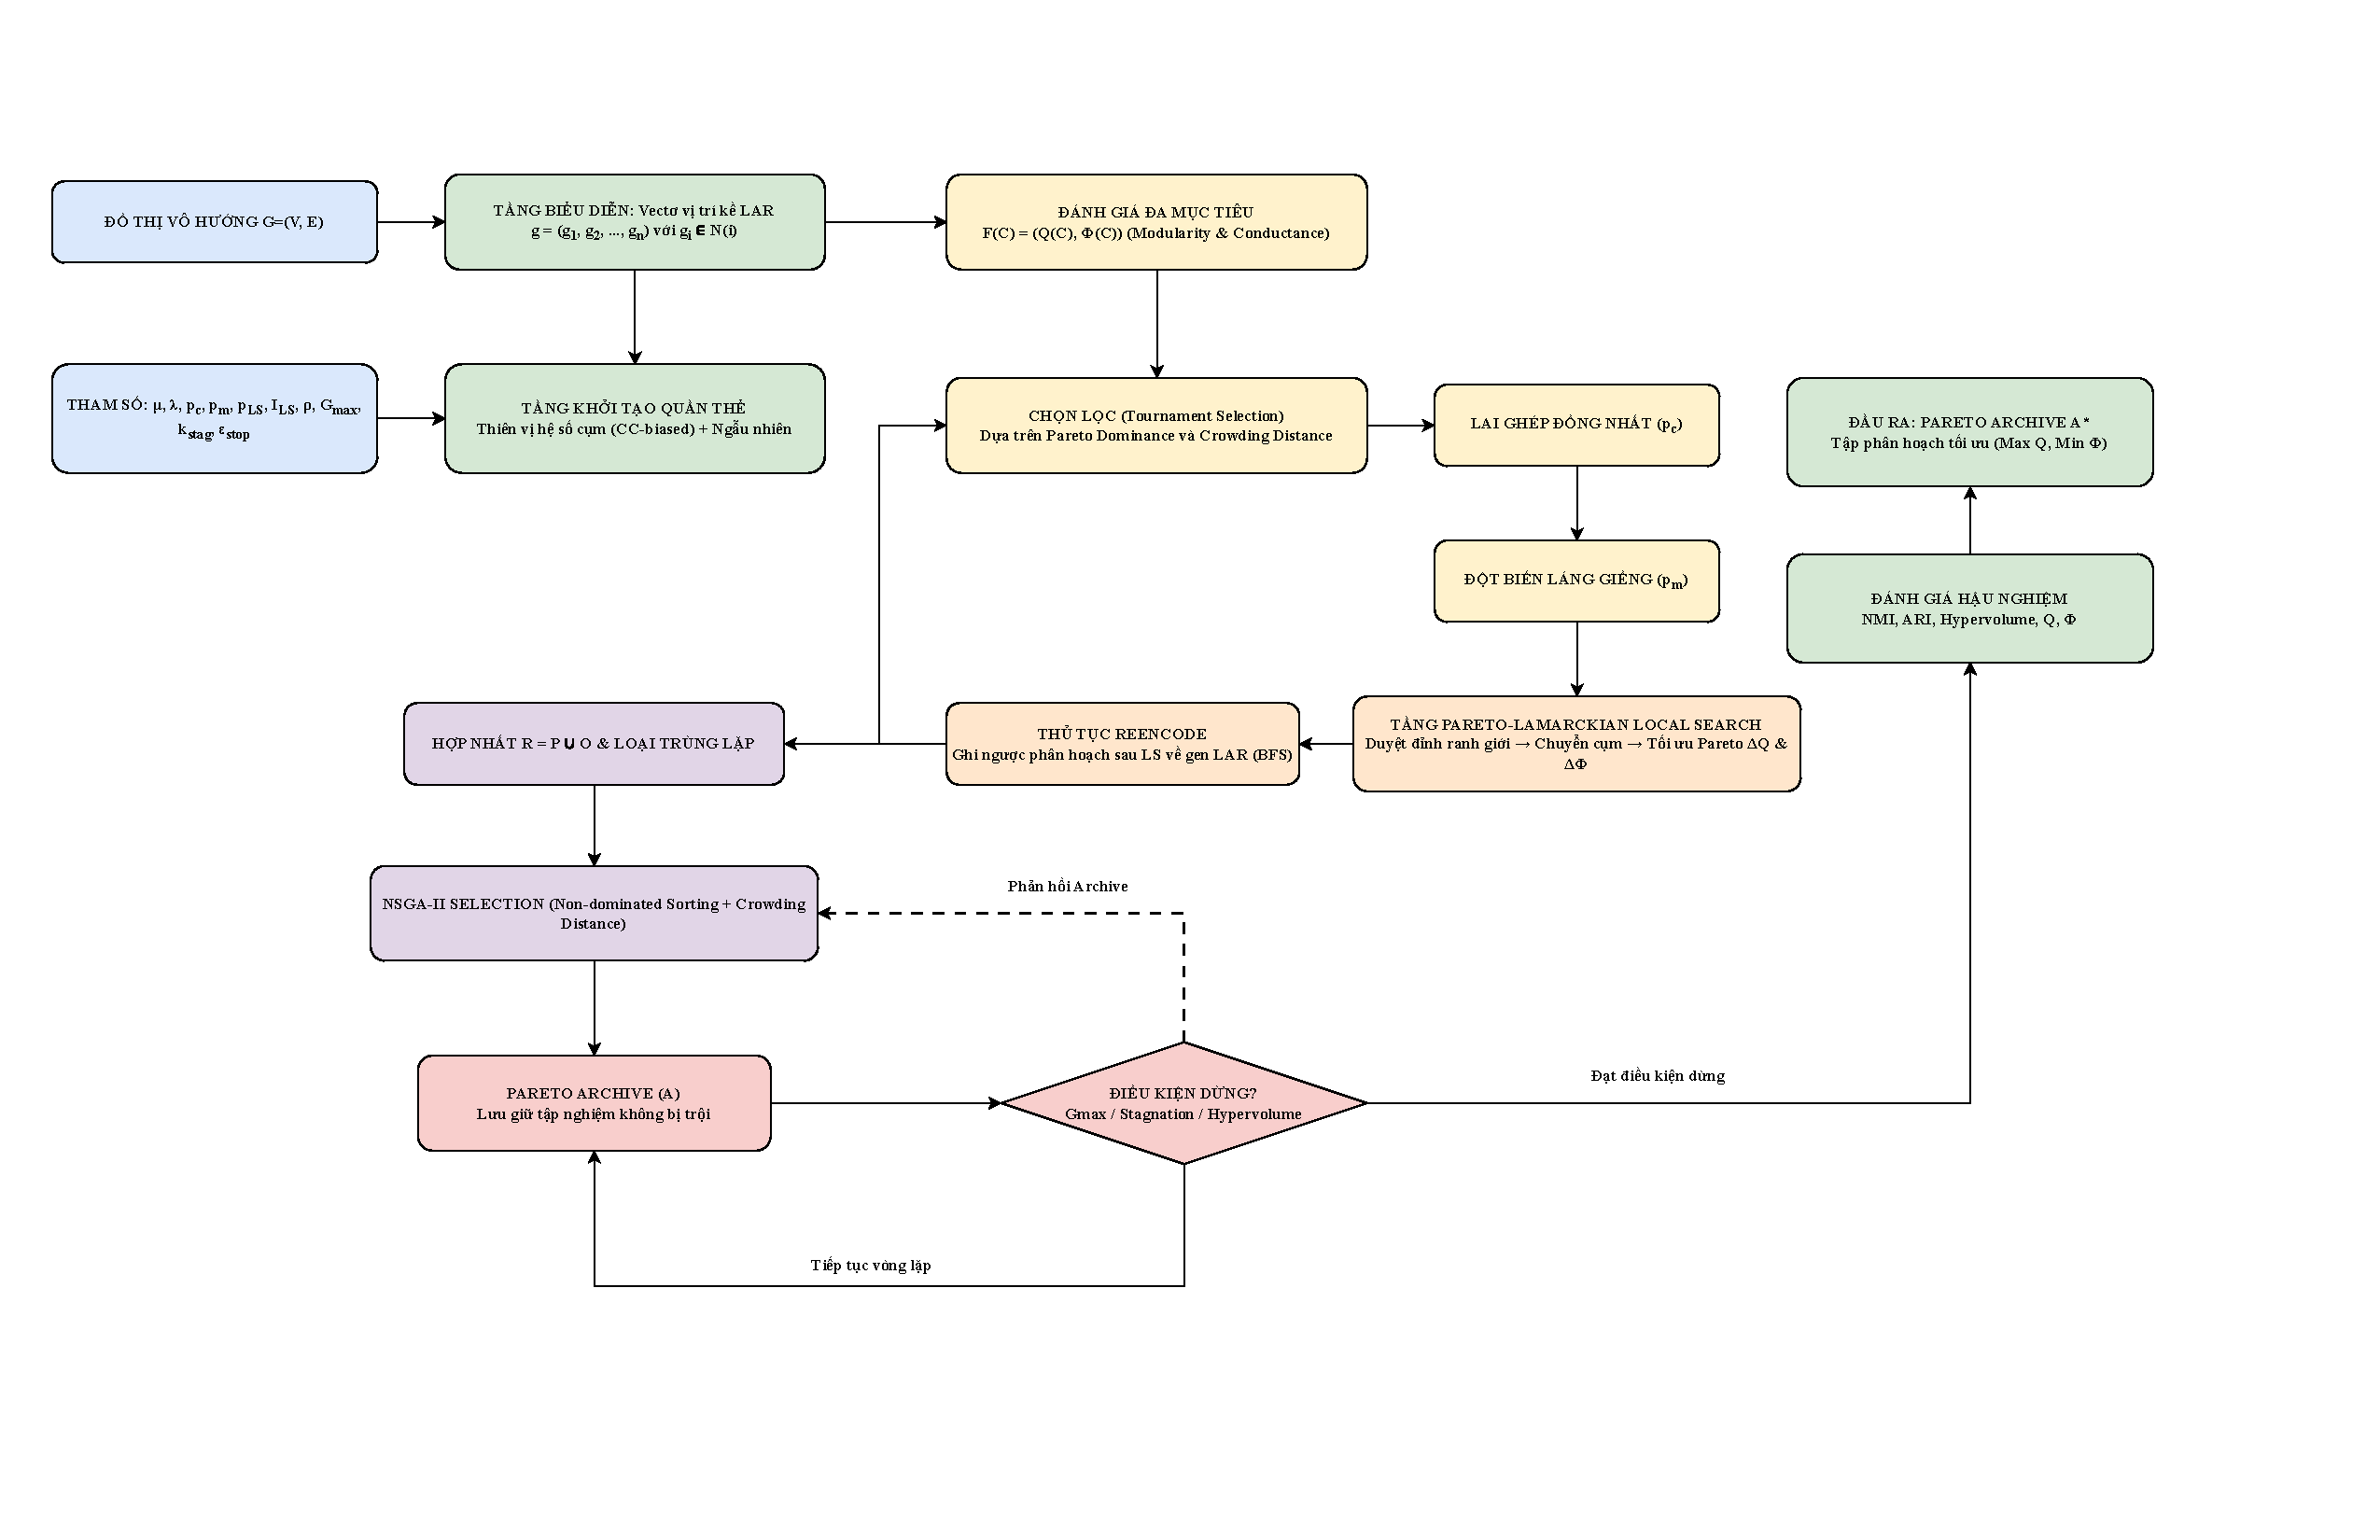
\includegraphics[width=1.0\textwidth]{diagram1.pdf} % Thay tên file của bạn vào đây
    \caption{Kiến trúc tổng thể của phương pháp MO-HGA-LS}
    \label{fig:architecture}
\end{figure}

Để tránh archive tăng không giới hạn, đặt kích thước tối đa $A_{\max}$. Khi $|\mathcal{A}|>A_{\max}$, các nghiệm có độ đóng góp đa dạng thấp hơn được loại bỏ theo chỉ số khoảng cách đám đông hoặc một quy tắc truncation được xác định trước.

\subsubsection{Quy trình hoạt động}

\begin{figure}[H]
    \centering
    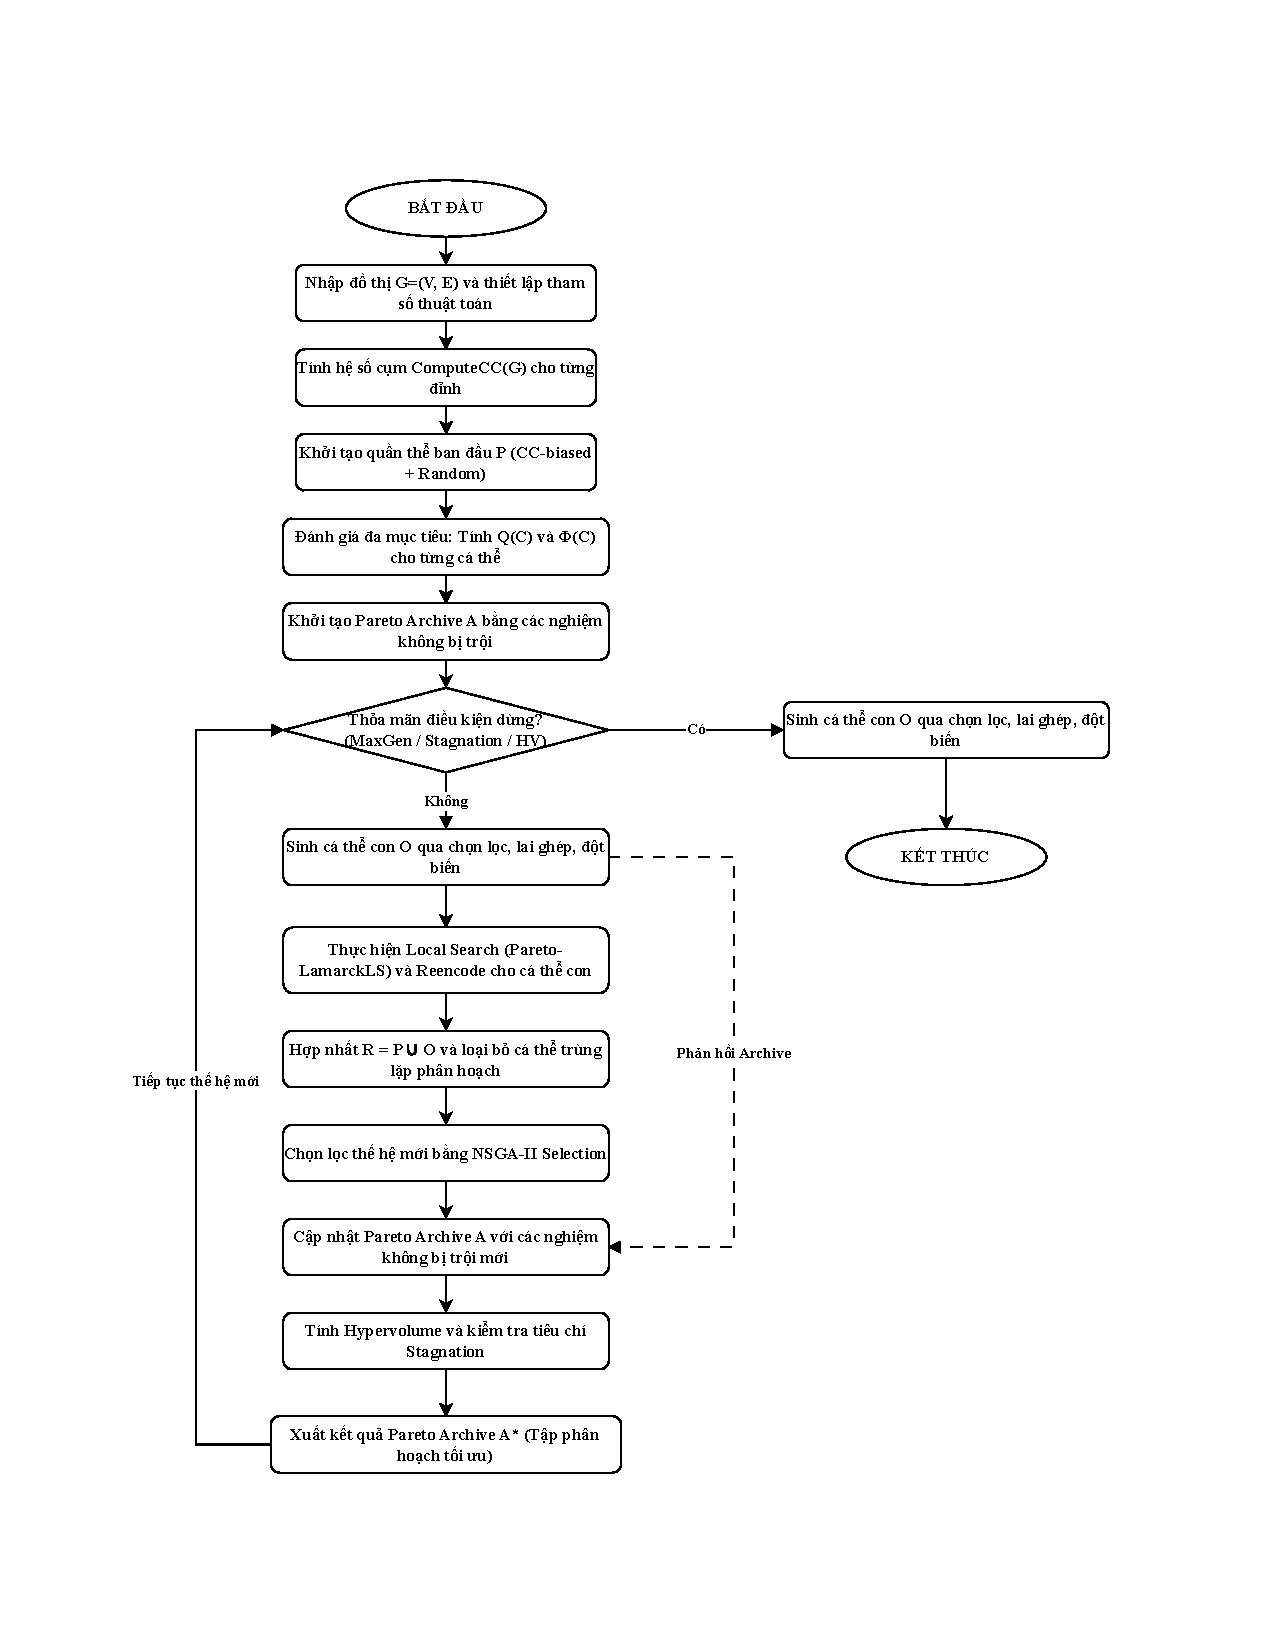
\includegraphics[width=1.0\textwidth]{diagram2.pdf}
    \caption{Lưu đồ hoạt động của MO-HGA-LS}
    \label{fig:flowchart}
\end{figure}

Quy trình của một thế hệ được thực hiện theo các bước sau:

\begin{enumerate}
    \item \textbf{Giải mã:} chuyển mỗi nhiễm sắc thể LAR thành phân hoạch bằng thành phần liên thông yếu của $G_g$.
    \item \textbf{Đánh giá:} tính $Q$ và $\Phi$ trên đồ thị gốc.
    \item \textbf{Sinh cá thể con:} áp dụng chọn lọc, lai ghép và đột biến.
    \item \textbf{Local Search:} với xác suất $p_{LS}$, thực hiện Pareto-Lamarck Local Search trên cá thể con.
    \item \textbf{Chọn thế hệ mới:} hợp quần thể cha và con, thực hiện non-dominated sorting và chỉ số khoảng cách đám đông để chọn $\mu$ cá thể.
    \item \textbf{Cập nhật archive:} hợp các nghiệm không bị trội vào archive và cắt giảm nếu vượt $A_{\max}$.
    \item \textbf{Kiểm tra dừng:} cập nhật Hypervolume và bộ đếm stagnation; dừng khi đạt $G_{\max}$ hoặc điều kiện trì trệ.
\end{enumerate}

\subsubsection{Thuật toán tổng quát}

Phần này trình bày chi tiết các mã giả cho thuật toán tổng quát MO-HGA-LS cùng các thủ tục bổ trợ bao gồm thuật toán tìm kiếm cục bộ đa mục tiêu Pareto-LamarckLS và thủ tục Reencode để ghi ngược cấu trúc phân hoạch về dạng biểu diễn gen.

\begin{algorithm}[H]
\caption{MO-HGA-LS}
\renewcommand{\alglinenumber}[1]{\normalsize #1.}
\begin{algorithmic}[1]
\Require Đồ thị $G$; $\mu,\lambda$; $p_c,p_m,p_{LS}$; $I_{LS}$; $\rho$; $A_{\max}$; $G_{\max},k_{\mathrm{stag}},\varepsilon_{\mathrm{stop}}$
\Ensure Pareto archive $\mathcal{A}$
\State $CC\leftarrow\mathrm{ComputeCC}(G)$
\State $\mathcal{P}\leftarrow\mathrm{InitPopulation}(G,CC,\mu,\rho)$
\State Xét $F(x)=(Q(x),\Phi(x))$ for $x\in\mathcal{P}$
\State $\mathcal{A}\leftarrow\mathrm{Truncate}(ND(\mathcal{P}),A_{\max})$
\State $gen\leftarrow0,\;stag\leftarrow0,\;HV_{\mathrm{best}}\leftarrow HV(\mathcal{A})$
\While{$gen<G_{\max}$ and $stag<k_{\mathrm{stag}}$}
    \State $\mathcal{O}\leftarrow\mathrm{GenerateOffspring}(\mathcal{P},\lambda,p_c,p_m,p_{LS},I_{LS})$
    \State Xét tất cả các partition mới trong $\mathcal{O}$
    \State $\mathcal{R}\leftarrow\mathcal{P}\cup\mathcal{O}$
    \State $\mathcal{P}\leftarrow\mathrm{NSGASelection}(\mathcal{R},\mu)$
    \State $\mathcal{A}\leftarrow\mathrm{Truncate}(ND(\mathcal{A}\cup\mathcal{O}),A_{\max})$
    \State $HV_{\mathrm{current}}\leftarrow HV(\mathcal{A})$
    \If{$HV_{\mathrm{current}}>HV_{\mathrm{best}}+\varepsilon_{\mathrm{stop}}$}
        \State $HV_{\mathrm{best}}\leftarrow HV_{\mathrm{current}}$
        \State $stag\leftarrow0$
    \Else
        \State $stag\leftarrow stag+1$
    \EndIf
    \State $gen\leftarrow gen+1$
\EndWhile
\State \Return $\mathcal{A}$
\end{algorithmic}
\end{algorithm}

Trong thuật toán trên, $\text{NSGASelection}$ thực hiện sắp xếp các cá thể theo Pareto front và sử dụng chỉ số khoảng cách đám đông để duy trì tính đa dạng khi số lượng cá thể trong một front vượt quá số vị trí còn lại của quần thể.

\begin{algorithm}[H]
\caption{Pareto-Lamarck Local Search}
\renewcommand{\alglinenumber}[1]{\normalsize #1.}
\begin{algorithmic}[1]
\Require Đồ thị $G$; cá thể $x$; số vòng lặp $I_{LS}$
\Ensure Cá thể $x'$
\State $\mathcal{C}\leftarrow\mathrm{Decode}(x)$
\State $\mathcal{A}_L\leftarrow\{\mathcal{C}\}$
\For{$it=1$ to $I_{LS}$}
    \State $\mathcal{B}\leftarrow\mathrm{Shuffle}(\mathrm{BoundaryVertices}(\mathcal{C}))$
    \State $moved\leftarrow\mathrm{false}$
    \For{each $u\in\mathcal{B}$}
        \State $\mathcal{N}\leftarrow\mathrm{EvaluateMoves}(G,\mathcal{C},u)$
        \State $\mathcal{N}^{*}\leftarrow ND(\{\mathcal{C}\}\cup\mathcal{N})$
        \State $\mathcal{A}_L\leftarrow ND(\mathcal{A}_L\cup\mathcal{N}^{*})$
        \If{$\mathcal{N}^{*}\setminus\{\mathcal{C}\}\neq\varnothing$}
            \State $\mathcal{C}\leftarrow\mathrm{SelectRepresentative}(\mathcal{N}^{*})$
            \State $moved\leftarrow\mathrm{true}$
        \EndIf
    \EndFor
    \If{not $moved$}
        \State \textbf{break}
    \EndIf
\EndFor
\State $\mathcal{C}^{*}\leftarrow\mathrm{SelectRepresentative}(\mathcal{A}_L)$
\State $x'\leftarrow\mathrm{Reencode}(G,\mathcal{C}^{*})$
\State \Return $x'$
\end{algorithmic}
\end{algorithm}

Trong thủ tục trên, $\mathrm{EvaluateMoves}$ chỉ sinh các phép chuyển đỉnh thỏa mãn ràng buộc khả thi. $\mathrm{SelectRepresentative}$ phải được định nghĩa cố định trong triển khai, chẳng hạn bằng khoảng cách tới điểm lý tưởng sau chuẩn hóa hoặc một tiêu chí knee-point. Nếu sử dụng chỉ số khoảng cách đám đông, cần ghi rõ rằng nó phục vụ lựa chọn nghiệm có tính đa dạng, không phải tối ưu tuyệt đối.

\begin{algorithm}[H]
\caption{Reencode}
\renewcommand{\alglinenumber}[1]{\normalsize #1.}
\begin{algorithmic}[1]
\Require Đồ thị $G$; phân hoạch liên thông $\mathcal{C}$
\Ensure Kiểu gen $g$
\For{each cộng đồng $C\in\mathcal{C}$}
    \State Chọn đỉnh gốc $r\in C$
    \State $T\leftarrow\mathrm{BFS}(G[C],r)$
    \For{each $u\in C\setminus\{r\}$}
        \State $g_u\leftarrow\mathrm{parent}_T(u)$
    \EndFor
    \State $g_r\leftarrow$ một láng giềng của $r$ trong $C$
\EndFor
\State \Return $g$
\end{algorithmic}
\end{algorithm}

Với điều kiện mỗi cộng đồng có ít nhất hai đỉnh và liên thông, Reencode tạo ra một cá thể LAR hợp lệ và giải mã lại đúng phân hoạch đầu vào. Chi phí thời gian là $\mathcal{O}(n+m)$.

% \subsubsection{Phân tích độ phức tạp tính toán}
% \subsection{Phân tích độ phức tạp thuật toán MO-HGA-LS}

\subsubsection{Phân tích độ phức tạp tính toán}

\noindent a) Độ phức tạp thời gian
\noindent \\ 
Chi phí tính toán cho các toán tử cốt lõi trong mỗi thế hệ được tổng hợp trong Bảng~\ref{tab:time_complexity}:

\begin{table}[H]
\centering
\begin{tabularx}{\textwidth}{|l|c|X|}
\hline
\textbf{Thành phần / Toán tử} & \makecell[c]{\textbf{Độ phức tạp}} & \textbf{Mô tả chi tiết} \\ \hline
Giải mã cá thể & $\mathcal{O}(n)$ & Dựa trên số lượng cung $n$ của đồ thị biểu diễn. \\ \hline
Đánh giá mục tiêu ($Q, \Phi$) & $\mathcal{O}(n + m)$ & Quét toàn bộ đồ thị với $n$ đỉnh và $m$ cạnh. \\ \hline
Hệ số gom cụm ($CC$) & $\mathcal{O}\left(\sum_{v\in V} k_v^2\right)$ & Tính trực tiếp theo số cặp láng giềng. \\ \hline
Tìm kiếm cục bộ (LS) & $\mathcal{O}(I_{LS} C_{LS})$ & Chi phí phụ thuộc vào \textit{incremental evaluation} ($C_{LS}$), thay vì gán cố định $\mathcal{O}(m)$. \\ \hline
Sắp xếp không trội & $\mathcal{O}(N^2)$ & Với kích thước gộp $N = \mu + \lambda$ và 2 mục tiêu. \\ \hline
Khoảng cách mật độ & $\mathcal{O}(N \log N)$ & Tính chỉ số khoảng cách đám đông trên mỗi front. \\ \hline
\end{tabularx}
\caption{Độ phức tạp thời gian của các thành phần trong MO-HGA-LS}
\label{tab:time_complexity}
\end{table}

\noindent Với giả định áp dụng đánh giá mục tiêu đầy đủ cho mọi cá thể, cận trên mang tính mô tả cho thời gian thực thi của thuật toán qua $G_{\max}$ thế hệ là:
\begin{equation*}
\mathcal{O}\left(
G_{\max}
\left[
(\mu+\lambda)(n+m)
+
\lambda p_{LS}I_{LS}C_{LS}
+
(\mu+\lambda)^2
\right]
\right)
\label{eq:time_bound}
\end{equation*}

Giá trị $C_{LS}$ phản ánh chi phí thực tế của thuật toán tìm kiếm cục bộ (sử dụng cập nhật chênh lệch) và không được thay thế tùy tiện bằng $m$.

\noindent b) Độ phức tạp không gian
\noindent \\ 
Nhu cầu bộ nhớ của thuật toán được phân bổ qua các cấu trúc dữ liệu chính như trong Bảng~\ref{tab:space_complexity}:

\begin{table}[H]
\centering
\begin{tabularx}{\textwidth}{|l|X|c|}
\hline
\textbf{Thành phần lưu trữ} & \textbf{Ký hiệu / Mô tả} & \makecell[c]{\textbf{Độ phức tạp không gian}} \\ \hline
Đồ thị ($G$) & Số đỉnh $n$, số cạnh $m$ & $\mathcal{O}(n + m)$ \\ \hline
Quần thể & Kích thước $\mu$ và $\lambda$ & $\mathcal{O}(\mu n)$ \\ \hline
Archive & Kích thước tối đa $A_{\max}$ & $\mathcal{O}(A_{\max} n)$ \\ \hline
\end{tabularx}
\caption{Độ phức tạp không gian của MO-HGA-LS}
\label{tab:space_complexity}
\end{table}

Do đó, việc thiết lập giới hạn cho kích thước tối đa của archive ($A_{\max}$) là bắt buộc nhằm kiểm soát hiệu quả bộ nhớ khi xử lý các mạng quy mô lớn.

\subsubsection{Thảo luận và định hướng đánh giá thực nghiệm}

MO-HGA-LS kết hợp ba cơ chế có vai trò khác nhau. GA đảm nhiệm khám phá không gian nghiệm; Local Search tăng cường khai thác vùng lân cận; tối ưu hóa Pareto duy trì các nghiệm thể hiện các mức đánh đổi giữa $Q$ và $\Phi$. Vì vậy, chi phí tính toán dự kiến cao hơn GA đơn mục tiêu do phải duy trì thứ tự Pareto, chỉ số khoảng cách đám đông và archive.

Một đóng góp cần được kiểm chứng bằng thực nghiệm là liệu việc kết hợp hai mục tiêu và Local Search có thực sự cải thiện chất lượng Pareto, độ ổn định và khả năng mở rộng so với các baseline hay không. Do đó, các phát biểu về mức cải thiện, tốc độ hội tụ hoặc tỷ lệ giảm số phép tìm kiếm chỉ được đưa ra sau khi có số liệu thực nghiệm.

\subsection{Thiết kế thực nghiệm}

\subsubsection{Bộ dữ liệu thực nghiệm}

\noindent a) Mô tả các bộ dữ liệu thực tế \\ \indent
Để đánh giá toàn diện hiệu năng của giải thuật đề xuất trên cả các mạng quy mô nhỏ (benchmark cơ bản) và mạng quy mô lớn (thực tế từ SNAP), thực nghiệm sử dụng 5 tập dữ liệu mạng lưới phổ biến sau:
\begin{itemize}
    \item \textbf{Zachary's Karate Club (Karate):}
    \begin{itemize}
        \item \textit{Mô tả:} Thu thập bởi Wayne W. Zachary, mô tả mối quan hệ giữa 34 thành viên của một câu lạc bộ võ thuật.
        \item \textit{Đặc điểm cấu trúc:} Đồ thị vô hướng, không trọng số với độ tập trung cụm cao. Do mâu thuẫn nội bộ, đồ thị phân tách thành 2 cộng đồng thực tế (ground-truth).
    \end{itemize}

    \item \textbf{Political Books (Polbooks):}
    \begin{itemize}
        \item \textit{Mô tả:} Thu thập bởi Valdis Krebs về mạng lưới đồng mua sách chính trị trên Amazon trước cuộc bầu cử tổng thống Mỹ năm 2004.
        \item \textit{Đặc điểm cấu trúc:} Gồm 105 nút (sách) và 441 cạnh (đồng mua), phân chia thành 3 cộng đồng thực tế chính: tự do (Liberal), bảo thủ (Conservative) và trung lập (Neutral).
    \end{itemize}

    \item \textbf{American College Football (Football):}
    \begin{itemize}
        \item \textit{Mô tả:} Mạng lưới các trận đấu bóng đá Mỹ cấp đại học giữa các đội tuyển trong mùa giải Division I-A năm 2000.
        \item \textit{Đặc điểm cấu trúc:} Gồm 115 nút và 613 cạnh, được phân chia tự nhiên thành 12 cộng đồng ứng với các liên đoàn thi đấu.
    \end{itemize}

    \item \textbf{SNAP Email-Eu-Core (Email):}
    \begin{itemize}
        \item \textit{Mô tả:} Thu thập từ dữ liệu email nội bộ của một viện nghiên cứu lớn tại Châu Âu, ghi nhận các trao đổi thông tin giữa các thành viên.
        \item \textit{Đặc điểm cấu trúc:} Gồm 1,005 nút và 25,571 cạnh với hệ số gom cụm trung bình 0.3994. Mỗi cá nhân thuộc chính xác một trong 42 phòng ban, tạo thành hệ thống cộng đồng thực tế.
    \end{itemize}

    \item \textbf{Amazon Co-purchasing Network (Amazon):}
    \begin{itemize}
        \item \textit{Mô tả:} Mạng lưới đồng mua sản phẩm trên nền tảng thương mại điện tử Amazon (thuộc SNAP).
        \item \textit{Đặc điểm cấu trúc:} Mạng quy mô lớn, thưa, với các cộng đồng thực tế phản ánh danh mục sản phẩm (product categories và sub-categories).
    \end{itemize}
\end{itemize}

\noindent b) Thông số cấu trúc của các bộ dữ liệu thực nghiệm \\ \indent
Bảng dưới đây tổng hợp chi tiết các thông số mạng của 5 bộ dữ liệu được sử dụng trong thực nghiệm:

%/////////////////////////////////////////
\begin{table}[H]
\centering
\begin{tabularx}{\textwidth}{|l|c|c|c|c|X|}
\hline
\textbf{Bộ dữ liệu} & \makecell[r]{\textbf{Số đỉnh}} & \makecell[r]{\textbf{Số cạnh}} & \makecell[c]{\textbf{Số bậc}\\\textbf{trung}\\\textbf{bình}} & \makecell[c]{\textbf{Hệ số}} & \textbf{Cộng đồng chuẩn} \\ \hline
Karate & 34 & 78 & 4.59 & 0.5706 & 2 nhóm (Rạn nứt CLB) \\ \hline
Polbooks & 105 & 441 & 8.40 & 0.4879 & 3 nhóm (Chính trị) \\ \hline
Football & 115 & 613 & 10.66 & 0.4034 & 12 nhóm (Liên đoàn) \\ \hline
Email & 1,005 & 25,571 & 50.89 & 0.3994 & 42 phòng ban viện nghiên cứu \\ \hline
Amazon & 334,863 & 925,872 & 5.53 & 0.3967 & Danh mục sản phẩm thương mại điện tử \\ \hline
\end{tabularx}
\caption{Thông số thống kê chi tiết của các bộ dữ liệu thực nghiệm}
\label{tab:datasets_info}
\end{table}

\subsubsection{Thiết lập tham số}

\noindent a) Nguyên tắc hiệu chỉnh tham số \\ \indent
Việc hiệu chỉnh tham số  đóng vai trò quyết định đến khả năng cân bằng giữa thăm dò toàn cục trong không gian tìm kiếm cấu trúc cộng đồng và khai thác cục bộ để tối ưu hóa giá trị hàm mục tiêu Modularity ($Q$).

\noindent b) Cấu hình chi tiết các tham số giải thuật \\ \indent
Các tham số của giải thuật được thiết lập cụ thể như sau:
\begin{itemize}
    \item kích thước quần thể $\mu=100$;
    \item số cá thể con $\lambda$ phải được ghi rõ trong mã nguồn/thực nghiệm;
    \item tỷ lệ lai $p_c=0.85$;
    \item tỷ lệ đột biến cơ sở $p_m=1/n$, cần kiểm tra độ nhạy trên mạng lớn;
    \item kích thước tournament $t=2$;
    \item số vòng Local Search tối đa $I_{LS}=30$;
    \item xác suất áp dụng Local Search $p_{LS}$ phải được công bố rõ;
    \item số thế hệ tối đa $G_{\max}=200$;
    \item ngưỡng trì trệ $\varepsilon_{\mathrm{stop}}$ và số thế hệ $k_{\mathrm{stag}}$ phải được cố định trước thực nghiệm;
    \item kích thước archive tối đa $A_{\max}$ phải được cố định và báo cáo.
\end{itemize}

Không nên mô tả các giá trị trên là tối ưu nếu chưa có quá trình hiệu chỉnh. Để tăng tính tin cậy, có thể thực hiện phân tích độ nhạy trên một tập dữ liệu hiệu chỉnh và giữ nguyên cấu hình được chọn cho các bộ dữ liệu đánh giá.

Mỗi cấu hình thuật toán nên được chạy độc lập ít nhất 20-30 lần với các seed khác nhau. Kết quả nên được báo cáo bằng trung bình độ lệch chuẩn hoặc trung vị và khoảng tứ phân vị, tùy phân bố dữ liệu.

\subsubsection{Các phương pháp baseline}

Để đánh giá đúng đóng góp của từng thành phần, nên sử dụng ít nhất các baseline sau:
\begin{itemize}
    \item \textbf{Louvain:} baseline heuristic tối ưu Modularity đa cấp \cite{Blondel2008}.
    \item \textbf{Leiden:} baseline heuristic cải tiến Louvain với cơ chế tinh chỉnh phân hoạch \cite{Traag2019}.
    \item \textbf{GA:} phiên bản GA sử dụng cùng LAR và các tham số chính nhưng không có Local Search.
    \item \textbf{MA-Q hoặc HGA-LS đơn mục tiêu:} phiên bản chỉ tối ưu Modularity, dùng để đánh giá tác động của Local Search và so sánh với bài toán đơn mục tiêu.
    \item \textbf{MOEA baseline:} NSGA-II hoặc một thuật toán đa mục tiêu tương đương với cùng hai mục tiêu $Q$ và $\Phi$, nếu khả năng cài đặt cho phép.
\end{itemize}

Việc sử dụng cùng cách tiền xử lý, cùng giới hạn tài nguyên và cùng số lần chạy độc lập là cần thiết để so sánh công bằng.

\subsubsection{Các tiêu chí đánh giá}

\noindent a) Đánh giá mục tiêu nội tại \\ \indent
$Q$ và $\Phi$ được dùng để đánh giá trực tiếp hai mục tiêu của thuật toán. Với thuật toán đa mục tiêu, không nên chỉ báo cáo một giá trị duy nhất mà nên trình bày Pareto front hoặc ít nhất các nghiệm đại diện.

\noindent b) Đánh giá chất lượng Pareto \\ \indent
Ba tiêu chí trên được kết hợp nhằm đánh giá kết quả một cách toàn diện, trong đó NMI và ARI tập trung vào mức độ phù hợp với phân hoạch tham chiếu, còn Modularity phản ánh chất lượng cấu trúc cộng đồng nội tại của mạng.

\noindent c) Đánh giá ngoại tại \\ \indent
NMI và ARI chỉ được tính trên các bộ dữ liệu có phân hoạch tham chiếu. Hai chỉ số này không tham gia tối ưu và được dùng để đánh giá mức độ tương đồng giữa nghiệm tìm được với partition chuẩn.

\noindent d) Đánh giá hiệu năng và độ ổn định \\ \indent
Báo cáo thời gian chạy, số thế hệ, số lần đánh giá hàm mục tiêu, kích thước archive và mức cải thiện HV theo thế hệ. Với các thuật toán ngẫu nhiên, báo cáo thống kê qua nhiều lần chạy và có thể sử dụng kiểm định thống kê phi tham số, chẳng hạn Wilcoxon signed-rank cho so sánh từng cặp, khi số liệu và thiết kế thí nghiệm đáp ứng điều kiện áp dụng.

\noindent e) Lựa chọn nghiệm cuối cùng \\ \indent
Vì MO-HGA-LS trả về một tập Pareto thay vì một nghiệm duy nhất, quy tắc chọn nghiệm cần được định nghĩa trước. Một lựa chọn phù hợp là báo cáo đồng thời:
\begin{itemize}
    \item nghiệm có $Q$ lớn nhất;
    \item nghiệm có $\Phi$ nhỏ nhất;
    \item nghiệm knee hoặc nghiệm gần điểm lý tưởng sau chuẩn hóa.
\end{itemize}
Nếu ứng dụng yêu cầu một phân hoạch duy nhất, phải nêu rõ tiêu chí lựa chọn và áp dụng nhất quán cho tất cả các phương pháp.

\subsection{Tóm tắt chương 2}
Chương 2 đã phát biểu bài toán phát hiện cộng đồng dưới dạng tối ưu hóa đa mục tiêu, trong đó $Q$ được cực đại hóa và Conductance trung bình $\Phi$ được cực tiểu hóa. Phương pháp MO-HGA-LS sử dụng biểu diễn LAR, khởi tạo thiên lệch theo hệ số phân cụm, các toán tử GA, Pareto-Lamarck Local Search và Pareto archive có giới hạn kích thước. Chương cũng làm rõ các điều kiện khả thi, cách cập nhật mục tiêu, độ phức tạp và thiết kế thực nghiệm. Các kết quả thực nghiệm, so sánh định lượng và phân tích thống kê cần được trình bày ở chương kết quả tương ứng; không suy diễn các mức cải thiện khi chưa có số liệu.

\newpage
\section{Phương pháp đề xuất cho bài toán phát hiện cộng đồng}

\renewcommand{\refname}{\mbox{Danh mục tài liệu tham khảo}}
\bibliographystyle{ieeetr}
\bibliography{baocao/latex/dacn}

\mbox{\textbf{\fontsize{14}{21}\selectfont Phụ lục}}


\addcontentsline{toc}{section}{Phụ lục}

\end{document}